%\documentclass[a4paper,fleqn,longmktitle]{cas-dc}
\documentclass[a4paper,fleqn]{cas-dc}

\usepackage{float}          % add
\usepackage{algorithm}      % add
\usepackage{algpseudocode}  % add
\usepackage{graphicx}       % add
\usepackage[numbers]{natbib}
%\usepackage[authoryear]{natbib}
%\usepackage[authoryear,longnamesfirst]{natbib}

%%%Author definitions
\def\tsc#1{\csdef{#1}{\textsc{\lowercase{#1}}\xspace}}

%%%

% Uncomment and use as if needed
%\newtheorem{theorem}{Theorem}
%\newtheorem{lemma}[theorem]{Lemma}
%\newdefinition{rmk}{Remark}
%\newproof{pf}{Proof}
%\newproof{pot}{Proof of Theorem \ref{thm}}

\begin{document}
\let\WriteBookmarks\relax
\def\floatpagepagefraction{1}
\def\textpagefraction{.001}

% Short title
\shorttitle{Parallel branch-and-bound for pump scheduling}

% Short author
\shortauthors{Souza et al.}

% Main title of the paper
\title [mode = title]{Parallel Branch-and-Bound for Exact Pump Scheduling with Constant-Time Hydraulic Backtracking}                      
% Title footnote mark
% eg: \tnotemark[1]

% Title footnote 1.
% eg: \tnotetext[1]{Title footnote text}
% \tnotetext[<tnote number>]{<tnote text>} 

% First author
%
% Options: Use if required
% eg: \author[1,3]{Author Name}[type=editor,
%       style=chinese,
%       auid=000,
%       bioid=1,
%       prefix=Sir,
%       orcid=0000-0000-0000-0000,
%       facebook=<facebook id>,
%       twitter=<twitter id>,
%       linkedin=<linkedin id>,
%       gplus=<gplus id>]

\author[1]{Michael Ferreira de Souza}
\ead{michael@ufc.br}
\credit{Conceptualization, Methodology, Software, Formal analysis, Investigation, Writing - Original draft}

\author[1]{Jéssica Gomes Melo da Rocha}
\cormark[2]
\ead{jessica@fisica.ufc.br}
\credit{Conceptualization, Methodology, Formal analysis, Validation, Writing - Review \& Editing}

\author[1]{Albert Einstein Fernandes Muritiba}
\ead{einstein@ufc.br}
\credit{Formal analysis, Validation, Visualization}

\author[1]{Ascânio Dias Araújo}
\cormark[1]
\ead{ascanio@fisica.ufc.br}
\credit{Supervision, Project administration}

\author[2]{Carlile Campos Lavor}
\ead{clavor@unicamp.br}
\credit{Supervision, Validation, Funding acquisition, Writing - Review \& Editing}

\affiliation[1]{
  organization={Universidade Federal do Ceará},
  addressline={Av. Mister Hull, s/n},
  city={Fortaleza},
  state={CE},
  postcode={60455-760},
  country={Brazil}
}

\affiliation[2]{
  organization={IMECC, Universidade Estadual de Campinas},
  addressline={Rua Sérgio Buarque de Holanda, 651},
  city={Campinas},
  state={SP},
  postcode={13083-859},
  country={Brazil}
}

\cortext[cor1]{Corresponding author. Email: ascanio@fisica.ufc.br}
\cortext[cor2]{Corresponding author. Email: jessica@fisica.ufc.br}

% Footnote text
%\fntext[fn1]{}

% For a title note without a number/mark
%\nonumnote{}

% Here goes the abstract (<= 250 palavras)
\begin{abstract}
  Pump scheduling in water distribution networks is a challenging combinatorial optimization problem that seeks to minimize energy costs while satisfying complex hydraulic constraints. Meta-heuristic approaches dominate the literature due to their flexibility but cannot guarantee global optimality. Exact methods such as Branch-and-Bound (B\&B) provide such guarantees but have historically been computationally prohibitive for realistic networks. This paper presents a scalable parallel B\&B framework incorporating three key innovations: MPI-based distributed computation, hydraulic snapshot persistence enabling constant-time state restoration during backtracking, and multi-criteria pruning within a depth-first search strategy. Integrated with a hydraulic simulation engine, the proposed solver reduces optimization time by one to two orders of magnitude compared to sequential implementations while maintaining optimality guarantees. Experimental results on a benchmark network demonstrate speedups of 29--115$\times$ and establish new best-known solutions relative to state-of-the-art meta-heuristics. These advances make exact pump scheduling practical for day-ahead operational planning in water distribution networks.
\end{abstract}

% Use if graphical abstract is present
% \begin{graphicalabstract}
% \includegraphics{figs/grabs.pdf}
% \end{graphicalabstract}

% Research highlights (3–5 bullets, até 85 caracteres cada)
\begin{highlights}
\item Parallel exact optimization for pump scheduling
\item Low-overhead hydraulic backtracking via state snapshots
\item Cooperative pruning accelerates convergence to global optimality
\item Efficient parallel search via deterministic load balancing
\item New best-known solutions for water distribution networks
\end{highlights}

% Keywords (1–7 keywords)
% Each keyword is seperated by \sep
\begin{keywords}
  pump scheduling \sep water distribution networks \sep branch-and-bound \sep parallel optimization \sep EPANET \sep combinatorial optimization
\end{keywords}

\maketitle

\section{Introduction}

Pump operations represent the dominant cost driver in water distribution networks (WDNs), with energy consumption for pumping comprising the largest share of operational expenses \cite{Paola2024}. As energy prices rise and environmental concerns intensify \cite{Reis2023}, developing efficient pump scheduling strategies has become both an economic and environmental imperative. Beyond cost minimization, effective scheduling influences system reliability, equipment longevity through controlled switching operations \cite{Lansey1994,Costa2016}, and service quality via consistent pressure maintenance and storage management \cite{Reis2023}.

The pump scheduling problem poses significant computational challenges. Decision variables are inherently discrete (pump on/off states), hydraulic constraints are nonlinear (pressure losses, pump curves), and operational requirements impose additional restrictions (tank level bounds, minimum pressures, maximum actuations). For a network with $N_p$ pumps over a 24-hour horizon, the solution space encompasses $2^{24 N_p}$ possible configurations. This combinatorial explosion, coupled with nonlinear hydraulic equations governing feasible solutions, places the problem firmly within the class of NP-hard mixed-integer nonlinear programs (MINLP) \cite{Fooladivanda2018,Verleye2016}.

Early research employed classical mathematical programming methods such as Linear Programming, Dynamic Programming, and Nonlinear Programming \cite{Brion1991,Jowitt1992}. While these methods yielded foundational insights, they struggled with the high dimensionality and non-convexity inherent to realistic networks \cite{Candelieri2018,Reis2023}. Dynamic programming, though theoretically elegant, remained confined to small networks lacking switching constraints \cite{Lansey1994}.

These computational barriers precipitated a paradigm shift toward meta-heuristics. Genetic Algorithms \cite{Savic1997,Mackle1995}, Ant Colony Optimization \cite{LpezIbez2008}, and Particle Swarm Optimization \cite{AlAni2012} emerged as dominant approaches \cite{Reis2023}, valued for their flexibility with discrete variables and complex constraint landscapes. However, all meta-heuristics share a fundamental limitation: they cannot guarantee optimality or quantify the gap to the global optimum \cite{Costa2016,Reis2023}. Recent innovations include Digital Harmony Search (DHS) \cite{Paola2024}, which incorporates real-time data with strict switching limits, and Smart Dynamic Local Search \cite{Bras2025}, employing duty-cycle formulations and perturbation mechanisms to escape local optima. Surrogate-based methods have also emerged to improve computational efficiency: Bayesian Optimization \cite{Candelieri2018,Bagloee2018} for reduced simulation calls, artificial neural network metamodels \cite{Broad2010,Rao2007} for accelerating hydraulic evaluations during optimization, and physics-informed graph neural networks \cite{Ashraf2024} for fast emulation of hydraulic simulators. Nevertheless, meta-heuristics require extensive parameter tuning and exhibit sensitivity to initial conditions \cite{Reis2023}.

The computational tractability of exact methods for realistic pump scheduling was an open question until Costa et al. \cite{Costa2016} demonstrated that Branch-and-Bound (B\&B) \cite{Land1960} could solve the problem for small-to-medium networks when appropriately constrained. Their key insight, which runs counter to typical assumptions, was that tighter operational constraints actually improve solver performance by enabling effective pruning of infeasible branches. In particular, limits on pump actuation frequency proved especially effective. However, their sequential implementation required hours or days of computation, limiting practical applicability. Recent efforts have also focused on developing tighter mathematical relaxations to improve B\&B performance. For instance, Bonvin et al. \cite{Bonvin2021} proposed a tailored Mixed-Integer Linear Programming (MILP) relaxation using Outer Approximation (OA) to handle the non-convex hydraulic laws, providing an exact method applicable to both fixed and variable-speed pumps. While they focus on mathematical tightness to prune the search space, scalability remains a primary bottleneck for exact methods \cite{Reis2023,MalaJetmarova2018}.

The increasing accessibility of computing clusters and mature distributed-memory frameworks has renewed interest in exact approaches. Parallel B\&B has proven successful in other combinatorial domains \cite{Gendron1994,Li1986,Hrga2021}, and decomposition methods like Generalized Benders Decomposition show promise for large networks with continuous relaxations \cite{Verleye2016}. Yet parallel B\&B for pump scheduling has remained limited \cite{Reis2023}, largely due to the computational overhead of repeated hydraulic simulations during tree traversal.

This work extends Costa et al.'s foundational approach \cite{Costa2016} with distributed-memory parallelism via MPI. We present a distributed-memory parallel B\&B solver combining MPI-based task parallelism, hydraulic state persistence for $O(1)$ backtracking, and a two-level schedule representation that reduces branching factors. Integrated with EPANET~3's improved computational engine, our framework delivers four principal contributions:
\begin{enumerate}
	\item A parallel task decomposition strategy with deterministic load balancing;
	\item A snapshot-based state management system eliminating redundant hydraulic simulations during backtracking;
	\item Cooperative pruning through non-blocking global bound synchronization;
	\item Empirical validation demonstrates that exact 24-hour solutions become computationally tractable, with runtimes reduced from days to hours.
\end{enumerate}

\section{Problem Formulation}

The pump scheduling problem is formulated as a mixed-integer nonlinear program (MINLP). The goal is to determine optimal ON/OFF schedules for all pumps over a fixed planning horizon, minimizing total energy costs while satisfying hydraulic and operational constraints.

\subsection{Notation}

\textbf{Sets:}
\begin{itemize}
	\item $\mathcal{H} = \{1, 2, \ldots, T\}$: Time steps in the planning horizon (typically $T = 24$ hours)
	\item $\mathcal{I}$: Network nodes (junctions and tanks)
	\item $\mathcal{K} \subseteq \mathcal{I}$: Storage tanks
	\item $\mathcal{A}$: Network arcs (directed links connecting nodes)
	\item $\mathcal{L} \subseteq \mathcal{A}$: Pipes
	\item $\mathcal{P} \subseteq \mathcal{A}$: Pumps, with $|\mathcal{P}| = N_p$
\end{itemize}

\textbf{Parameters:}
\begin{itemize}
	\item $C_{j,h}$: Electricity tariff for pump $j$ at time $h$ (\$/kWh)
	\item $P_{i}^{\min}, P_{i}^{\max}$: Pressure bounds at node $i$ (m)
	\item $L_{k}^{\min}, L_{k}^{\max}$: Water level bounds for tank $k$ (m)
	\item $L_{k,0}$: Initial water level in tank $k$
	\item $NA_{\max}$: Maximum pump state transitions (ON$\to$OFF or OFF$\to$ON) per pump per day
\end{itemize}

\textbf{Decision Variables:}
\begin{itemize}
	\item $x_{j,h} \in \{0, 1\}$: Binary status of pump $j$ at hour $h$ (1 = ON, 0 = OFF)
\end{itemize}

\subsection{Objective Function}

The objective minimizes total energy cost over the planning horizon:
\begin{equation}
	\min_{\mathbf{x}} \quad z = \sum_{h=1}^{T} \sum_{j \in \mathcal{P}} C_{j,h} \cdot E_{j,h}(\mathbf{x})
\end{equation}
where $E_{j,h}(\mathbf{x})$ denotes the energy consumed by pump $j$ during hour $h$, obtained from hydraulic simulation based on the full schedule $\mathbf{x}$.

\subsection{Constraints}

\textbf{Nodal Pressure Limits.} Pressures must remain within bounds to ensure adequate service without risking pipe damage:
\begin{equation}
	P_{i}^{\min} \le P_{i,h}(\mathbf{x}) \le P_{i}^{\max} \quad \forall i \in \mathcal{I}, \; \forall h \in \mathcal{H}
	\label{eq:pressure_limits}
\end{equation}

\textbf{Tank Storage Bounds.} Water levels must stay within operational limits to prevent overflow or depletion:
\begin{equation}
	L_{k}^{\min} \le L_{k,h}(\mathbf{x}) \le L_{k}^{\max} \quad \forall k \in \mathcal{K}, \; \forall h \in \mathcal{H}
	\label{eq:tank_bounds}
\end{equation}

\textbf{Tank Recovery.} To ensure day-to-day sustainability, final tank levels must meet or exceed initial levels:
\begin{equation}
	L_{k,T}(\mathbf{x}) \ge L_{k,0} \quad \forall k \in \mathcal{K}
	\label{eq:tank_recovery}
\end{equation}

\textbf{Actuation Limits.} To reduce mechanical wear and maintenance costs, pump switching is restricted:
\begin{equation}
	\sum_{h=2}^{T} |x_{j,h} - x_{j,h-1}| \le NA_{\max} \quad \forall j \in \mathcal{P}
	\label{eq:actuation_limits}
\end{equation}

\textbf{Hydraulic Model.} The hydraulic state is governed by physical laws governing flow conservation, head losses, and pump characteristics \cite{Bonvin2021}. Let $q_{a,h} \in \mathbb{R}$ denote the flow rate (m$^3$/h) through arc $a$ at hour $h$, and $H_{i,h} \geq 0$ denote the hydraulic head (m) at node $i$, defined as the sum of elevation and pressure head.

Flow conservation at each internal node requires:
\begin{multline}
	\sum_{a \in \delta^-(j)} q_{a,h} - \sum_{a \in \delta^+(j)} q_{a,h} = D_{j,h}, \\
	\quad \forall j \in \mathcal{I} \setminus \mathcal{K}, \; \forall h \in \mathcal{H}
	\label{eq:flow_conservation}
\end{multline}
where $\delta^-(j)$ and $\delta^+(j)$ denote arcs entering and leaving node $j$, respectively, and $D_{j,h} \geq 0$ is the water demand rate at node $j$ during hour $h$.

For each pipe $\ell = (i,j) \in \mathcal{L}$, head loss follows the Hazen-Williams or Darcy-Weisbach relationship \cite{Brown2002,Burgschweiger2009a}:
\begin{equation}
	H_{i,h} - H_{j,h} = \Phi_\ell(q_{\ell,h}), \quad \forall \ell \in \mathcal{L}, \; \forall h \in \mathcal{H}
	\label{eq:pipe_head_loss}
\end{equation}
where $\Phi_\ell(\cdot)$ is a nonlinear function with $\Phi_\ell(0) = 0$ and $\text{sgn}(\Phi_\ell(q)) = \text{sgn}(q)$ for all $q$.

For each pump $p = (i,j) \in \mathcal{P}$, the head increase across the pump depends on its status and flow \cite{Burgschweiger2009b,Morsi2012}:
\begin{multline}
	H_{j,h} - H_{i,h} = \Psi_p(q_{p,h}) \cdot x_{p,h}, \\
	\quad \forall p \in \mathcal{P}, \; \forall h \in \mathcal{H}
	\label{eq:pump_head}
\end{multline}
where $\Psi_p(\cdot)$ is the pump curve derived from manufacturer data, and $x_{p,h} \in \{0,1\}$ is the binary pump status.

Tank dynamics relate net inflow to water level change:
\begin{multline}
	\sum_{a \in \delta^-(k)} q_{a,h} - \sum_{a \in \delta^+(k)} q_{a,h} = \frac{S_k}{\Delta t} (L_{k,h} - L_{k,h-1}), \\
	\forall k \in \mathcal{K}, \; \forall h \in \mathcal{H}
	\label{eq:tank_dynamics}
\end{multline}
where $S_k$ is the tank cross-sectional area (m$^2$) and $\Delta t = 1$ hour.

Rather than explicitly encoding the nonlinear constraints \eqref{eq:flow_conservation}--\eqref{eq:tank_dynamics} in the optimization, our approach evaluates feasibility through hydraulic simulation. For each candidate schedule $\mathbf{x}$ visited during Branch-and-Bound traversal, EPANET~3 computes the hydraulic state (flows, heads, tank levels) by solving the full system \eqref{eq:flow_conservation}--\eqref{eq:tank_dynamics} using the Global Gradient Algorithm \cite{Todini1988}. We then enforce constraints \eqref{eq:pressure_limits}, \eqref{eq:tank_bounds}, and \eqref{eq:tank_recovery} based on these simulated values. The actuation constraint \eqref{eq:actuation_limits} is enforced directly during schedule construction.

While this simulation-based approach ensures hydraulic accuracy, it introduces a computational bottleneck: each node in the Branch-and-Bound search tree requires a complete hydraulic simulation, and the number of nodes grows exponentially with the planning horizon. For a 24-hour schedule with $NA_{\max}=3$, the search tree may contain billions of nodes, making sequential enumeration impractical. The following section addresses this challenge through parallelization and algorithmic optimizations that reduce both the number of nodes explored and the cost per node.

\section{Enhanced Branch-and-Bound}

We present a distributed-memory parallel Branch-and-Bound (B\&B) algorithm integrated with the EPANET~3 hydraulic engine. We adopt the two-level schedule representation proposed by Costa et al. \cite{Costa2016}, minimizing the branching factor, but enhance it with a Least Used Selection (LUS) strategy. To address scalability limitations of prior exact methods, we introduce three architectural innovations: cost-based pruning (which was not utilized in \cite{Costa2016}), MPI-based static load balancing with cooperative pruning, and a hydraulic snapshot mechanism for $O(1)$ state restoration.

\subsection{Two-Level Schedule Representation}

To mitigate the $2^{N_p \times T}$ combinatorial explosion, we adopt the variable separation strategy of Costa et al. \cite{Costa2016}. A high-level decision variable $y_h \in \{0, 1, \dots, N_p\}$ represents the number of active pumps at hour $h$. The low-level binary configuration $\mathbf{x}_h = \{x_{1,h}, \dots, x_{N_p,h}\}$ is derived from $y_h$ via a deterministic greedy mapping:
\[
	\mathcal{M}: (y_h, \mathbf{x}_{h-1}, \mathcal{R}) \to \mathbf{x}_h
\]
where $\mathcal{R}$ denotes the remaining actuation budget for each pump. Figure~\ref{fig:two_level} illustrates this representation: the high-level schedule $y_h$ specifies that 2, 3, 3, 2, 1, and 0 pumps should be active over six hours, which the mapping $\mathcal{M}$ converts into explicit binary pump states $x_{j,h}$.

\begin{figure}[htbp]
	\centering
	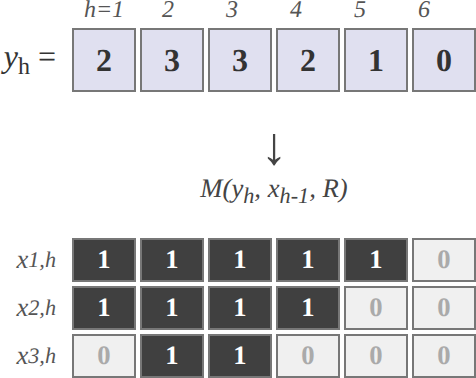
\includegraphics[width=0.7\columnwidth]{figures/Figure_1_two_level_diagram.png}
	\caption{Two-level schedule representation. The high-level variable $y_h$ indicates how many pumps are active at each hour (here: 2, 3, 3, 2, 1, 0 over six hours for three pumps). The mapping $\mathcal{M}$ derives binary configurations $x_{j,h}$ respecting actuation constraints.}
	\label{fig:two_level}
\end{figure}

The mapping $\mathcal{M}$ selects pumps to satisfy the target count $y_h$ while respecting actuation constraints $NA_{\max}$. Costa et al.\ \cite{Costa2016} employ a \emph{sequential exhaustion} strategy: pump $j$ is used exclusively until it exhausts its actuation budget, at which point the algorithm switches to pump $j+1$. For instance, with one active pump, the sequence proceeds as $(1,0,0) \to (0,1,0) \to (0,0,1)$. Each pump operates until depleted before ceding to the next.

We propose \emph{Least Used Selection} (LUS), which instead sorts pumps dynamically at each decision point by their remaining actuation budget. When switching pumps on, the algorithm prioritizes those with the most remaining on-switches; when switching off, it favors those with the most remaining off-switches. This greedy reordering serves a dual purpose: extending equipment life through balanced utilization across the pump station, while increasing the probability of finding feasible schedule extensions deeper in the search tree by preserving actuation flexibility.

\subsection{Task Decomposition and Parallel Execution}

We decompose the search tree into independent sub-problems to exploit distributed-memory parallelism. Each \emph{task} is defined by a fixed prefix of the high-level schedule, $\mathbf{y}_{1:L} = \{y_1, \dots, y_L\}$, where $L$ denotes the decomposition level (typically $L=8$). This yields $(N_p + 1)^L$ total tasks. Figure~\ref{fig:tree_decomposition} illustrates this decomposition: prefixes are enumerated at level $L$, and each resulting subtree is assigned to an MPI rank for independent exploration.

\begin{figure}[htbp]
	\centering
	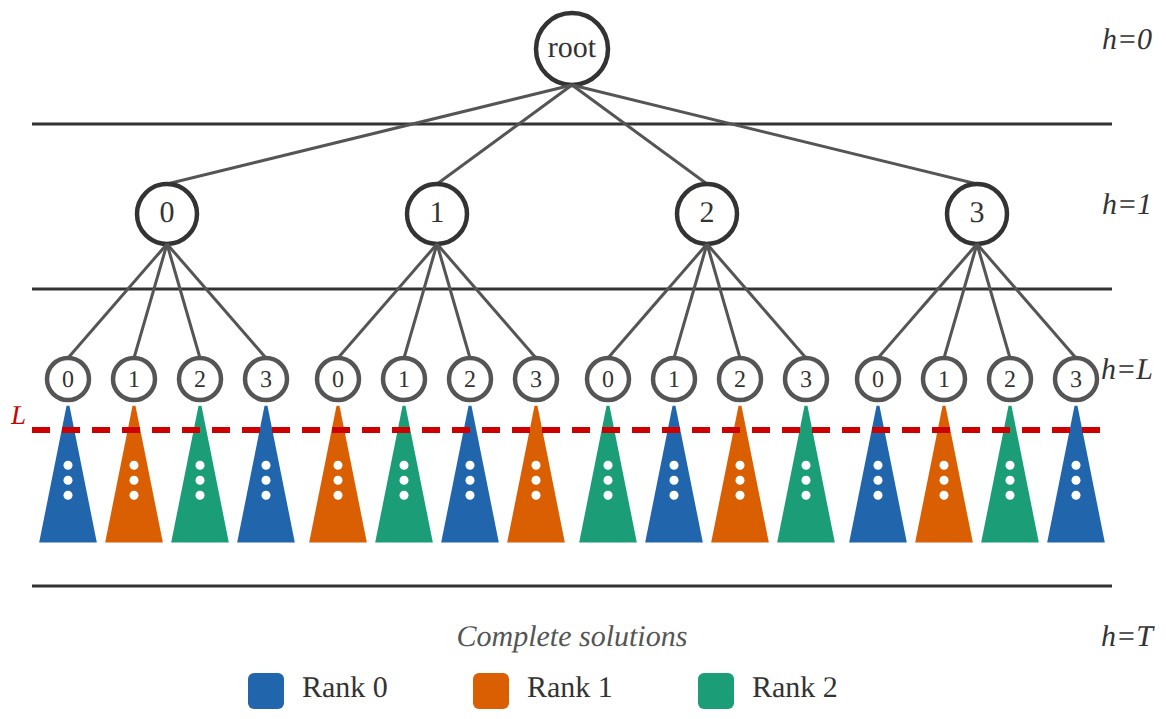
\includegraphics[width=0.9\columnwidth]{figures/Figure_2_tree_decomposition.png}
	\caption{Task decomposition by prefix. The search tree is partitioned at level $L$, yielding $(N_p+1)^L$ independent subtrees distributed across MPI ranks. In this example, $L=2$ and $N_p=3$ generate 16 tasks assigned to 3 ranks via round-robin.}
	\label{fig:tree_decomposition}
\end{figure}

To achieve load balancing without the overhead of dynamic work stealing, we employ deterministic hashing: tasks are enumerated and assigned round-robin based on a hash of their prefix:
\begin{equation}
	\text{Rank}(task_i) = \text{hash}(i) \mod N_{\text{procs}}
\end{equation}
This approach mitigates the irregular structure of B\&B trees, where some branches prune early while others require deep exploration.

Cooperative pruning leverages non-blocking global bound synchronization. Each process maintains a local upper bound $UB_{\text{local}}$ and periodically exchanges information via MPI collective operations to compute the global minimum $UB_{\text{global}}$. This enables processes to prune sub-optimal branches based on solutions discovered by remote peers.

\subsection{Hydraulic Snapshot Persistence}

A critical bottleneck in simulation-based optimization is constraint evaluation cost. Standard Extended Period Simulation (EPS) requires simulating from $t=0$ to $t=h$ to determine the hydraulic state at hour $h$. In depth-first traversal, backtracking from hour $h$ to $h-1$ traditionally necessitates complete re-simulation---an expensive operation repeated potentially billions of times during tree exploration.

EPANET~3 does not natively support state persistence for mid-simulation restoration. We therefore extended the hydraulic engine with a hierarchical snapshot mechanism that captures the minimal state required to resume simulation from any hour boundary. A \emph{snapshot} $S_h$ is a lightweight data structure storing:
\begin{description}
	\item[Node states:] hydraulic heads, demands, and outflows at all junctions;
	\item[Tank states:] water volumes and surface areas;
	\item[Link states:] flow rates, head losses, and valve/pump settings;
	\item[Pump energy accumulators:] cumulative kWh consumption and operating costs;
	\item[Solver state:] current simulation time, time pattern indices, and iterative solver variables.
\end{description}
Structural data (network topology, curves, control rules) remain in memory and are not duplicated. This design keeps snapshots compact while enabling complete state restoration.

During tree traversal, a snapshot is saved after each feasible hour:
\begin{equation}
	S_h = \textsc{Save}(\textsc{Simulate}(S_{h-1}, \mathbf{x}_h))
\end{equation}
Backtracking to explore alternative branches at hour $h-1$ reduces to a memory copy, $S_{h-1} \to \text{CurrentState}$, which executes in $O(1)$ relative to simulation time. The \textsc{Save} and \textsc{Load} operations in Algorithm~\ref{alg:bb_solver} (lines 17 and 20) implement this mechanism. Table~\ref{tab:ablation} shows that snapshot persistence delivers a 10.1$\times$ speedup by eliminating redundant hydraulic computations.

However, snapshot-based backtracking alone is insufficient for exact optimization if the hydraulic solver introduces path-dependent variability. EPANET's Global Gradient Algorithm uses an iterative Newton-Raphson method whose initial guess depends on the preceding hydraulic state. With the default convergence tolerance of $\epsilon = 10^{-3}$, identical pump configurations $y_h$ reached via different search trajectories can produce energy discrepancies of up to 0.03~kWh. Such numerical noise violates the requirement that costs depend solely on the current configuration, undermining pruning guarantees.

To eliminate path-dependency, we tighten the solver tolerance to $\epsilon = 10^{-7}$ for all experiments. This ensures that the hourly cost $\sum_j C_{j,h} \cdot E_{j,h}(S_{h-1}, \mathbf{x}_h)$ is numerically consistent across all search paths reaching the same state, restoring strict cost determinism necessary for provable optimality.

\subsection{Algorithm and Pruning Strategies}

A key property enabling effective pruning is the \emph{monotonicity} of the objective function. Because energy consumption $E_{j,h} \ge 0$ and electricity tariffs $C_{j,h} \ge 0$, each hourly cost contribution is non-negative. Consequently, the accumulated cost up to hour $h$, $z_h$,
\[
	z_h = \sum_{t=1}^{h} \sum_{j=1}^{N_p} C_{j,t} \cdot E_{j,t},
\]
is monotonically non-decreasing as the search progresses: $z_h \le z_{h+1} \le \cdots \le z_T$. This guarantees that if a partial solution's cost already meets or exceeds the best known complete solution, no extension of that partial solution can improve upon it. The branch can therefore be safely pruned without loss of optimality.

Our solver employs Depth-First Search (DFS), applying the following pruning criteria at each node (hour $h$) in order of computational cost:
\begin{enumerate}
	\item \textbf{Actuation Viability:} Prune if $y_h \to \mathbf{x}_h$ mapping is infeasible within remaining budgets.
	\item \textbf{Tank Bounds:} Prune if $L_{k,h} \notin [L_{k}^{\min}, L_{k}^{\max}]$ for any tank $k$.
	\item \textbf{Cost Bound:} Prune if $z_h \ge UB_{\text{global}}$, since monotonicity ensures no feasible extension can yield a lower total cost.
	\item \textbf{Pressure Limits:} Prune if $P_{i,h} < P_{i}^{\min}$ for any node $i$.
	\item \textbf{Tank Recovery} (at $h=T$ only): Prune if $L_{k,T} < L_{k,0}$ for any tank $k$. Intermediate schedules are not pruned on this criterion because tank levels may still recover through subsequent pump operations.
\end{enumerate}
This ordering prioritizes inexpensive checks (actuation, bounds) before hydraulic simulation, maximizing pruning efficiency. Algorithm~\ref{alg:bb_solver} outlines the complete parallel procedure, which consists of two phases: a static distribution of search space prefixes to MPI ranks (Lines 1--8), followed by a recursive Depth-First Search (DFS) for each assigned task. Here, $z^*$ denotes the global upper bound shared across processes (i.e., $z^* \equiv UB_{\text{global}}$), $S_h$ represents the hydraulic snapshot at hour $h$, and $c$ is the accumulated cost. The auxiliary function \textsc{Map} handles the greedy variable separation $\mathcal{M}$, while \textsc{Sim} performs hydraulic simulation to verify constraints: \textsc{Sim}($\mathbf{y}_{1:L}$) simulates the entire prefix to initialize a task, and \textsc{Sim}($h, \mathbf{x}_h$) advances simulation by one hour. State management is handled by \textsc{Save} and \textsc{Load}, which enable $O(1)$ backtracking by storing and restoring hydraulic snapshots.

Our choice of DFS over the Breadth-First Search (BFS) strategy employed by Costa et al. \cite{Costa2016} is deliberate: DFS discovers complete feasible solutions more rapidly, establishing an upper bound sooner for effective cost-based pruning. Furthermore, DFS requires only $O(\text{depth})$ memory compared to $O(\text{width})$ for BFS, which is essential for parallel scalability across distributed-memory systems.

\begin{algorithm}
	\footnotesize
	\caption{Parallel Branch-and-Bound}
	\label{alg:bb_solver}
	\begin{algorithmic}[1]
		\Require Horizon $T$, Decomposition level $L$, MPI rank $r$
		\State $\mathcal{T} \gets \{t \in \text{Prefixes}(L) \mid \text{hash}(t) \mod N_{\text{procs}} = r\}$
		\State $z^* \gets \infty$
		\For{each prefix $\mathbf{y}_{1:L}$ in $\mathcal{T}$}
		\State $S_L, c_L \gets \Call{Sim}{\mathbf{y}_{1:L}}$
		\If{$S_L$ feasible} \Call{DFS}{$L+1, S_L, c_L$} \EndIf
		\State \Call{Sync}{} \Comment{Non-blocking MPI bound exchange}
		\EndFor

		\Procedure{DFS}{$h, S, c$}
		\If{$c \ge z^*$} \Return \EndIf
		\If{$h > T$}
		\If{tanks recovered} $z^* \gets c$; \Call{Sync}{} \EndIf
		\Return
		\EndIf
		\For{$y = 0$ to $N_p$} \Comment{$y$ = target active pump count}
		\State $\mathbf{x}_h \gets \Call{Map}{y}$
		\If{$\mathbf{x}_h$ invalid} \textbf{continue} \EndIf
		\State $S_h, f \gets \Call{Sim}{h, \mathbf{x}_h}$
		\If{$f$}
		\State \Call{Save}{$S_h$}
		\State \Call{DFS}{$h{+}1, S_h, c{+}c_h$}
		\EndIf
		\State \Call{Load}{$S$}
		\EndFor
		\EndProcedure
	\end{algorithmic}
\end{algorithm}

Having described our parallel B\&B framework, we now validate its performance through systematic experiments on a standard benchmark network, examining scalability, ablation effects, and comparison with prior methods.

\section{Numerical Experiments}

The solver was implemented in C++17 with MPI for distributed computation. All experiments ran on a Linux server with an AMD EPYC 9554 64-Core Processor (128 logical cores with SMT enabled) and 384~GB RAM. Code was compiled using Intel oneAPI DPC++/C++ Compiler 2025.3.1 with \texttt{-O3 -march=native -flto} optimization flags. Hydraulic simulations used a customized EPANET~3.0 library.

\subsection{Case Study Network}

To evaluate solver performance, we employ the AnyTown Modified network, a well-established benchmark in pump scheduling research. This network was originally proposed by Walski et al. \cite{Walski1987} and subsequently modified by Rao and Salomons \cite{Rao2006} to increase optimization complexity. The modified network comprises 44 pipes, 25 nodes, and three storage tanks located at nodes 65, 165, and 265. Water is supplied from a source at node 10 through three identical fixed-speed pumps operating in parallel (111, 222, and 333). All demand nodes follow the same temporal pattern, scaled by individual demand multipliers. Storage tanks operate within level bounds of 66.53 m (minimum) and 71.53 m (maximum). Figure~\ref{fig:anytown_network} shows the network topology used in our experiments, and Figure~\ref{fig:anytown_energy_cost} shows the hourly energy price pattern used for pump operating costs. This benchmark is particularly valuable for benchmarking because it captures the essential features of real-world systems (multiple pumps, storage facilities, and time-varying demands) while remaining tractable for comprehensive optimization studies.

\begin{figure}[htbp]
	\centering
	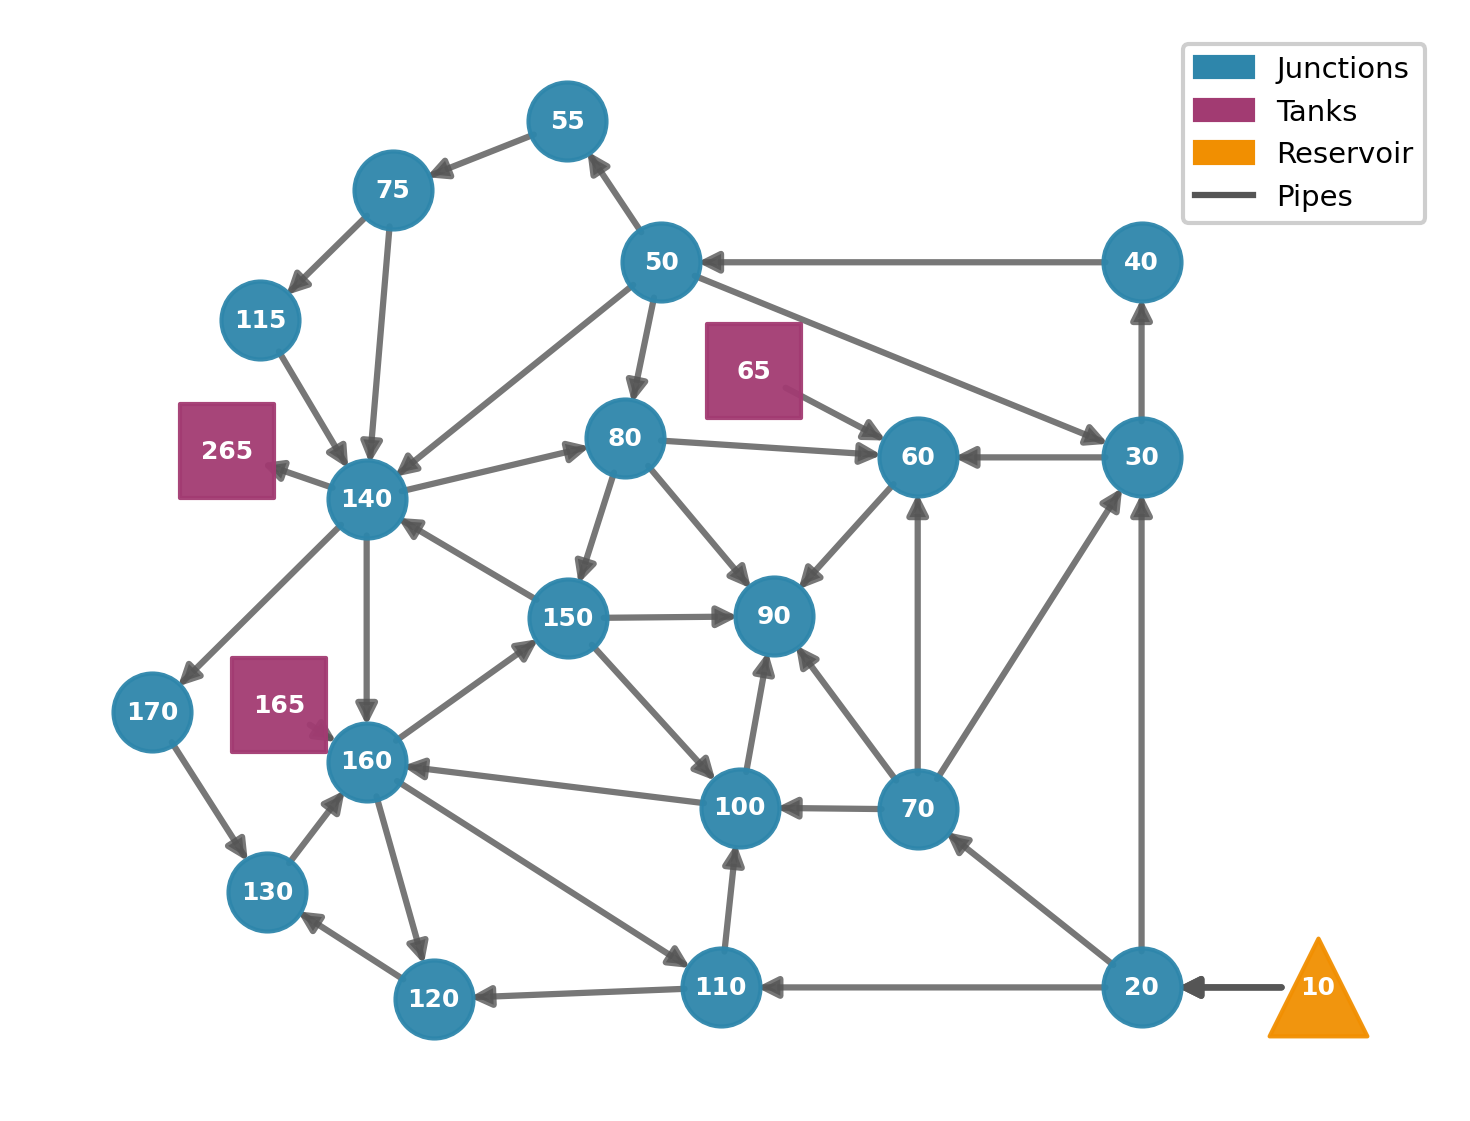
\includegraphics[width=0.9\columnwidth]{figures/Figure_3_anytown_network.png}
	\caption{Topology of the AnyTown Modified network. The network includes a reservoir (node 10), three storage tanks (nodes 65, 165, 265), and 19 demand nodes connected by 44 pipes. Three parallel pumps supply water from the reservoir.}
	\label{fig:anytown_network}
\end{figure}

\begin{figure}[htbp]
	\centering
	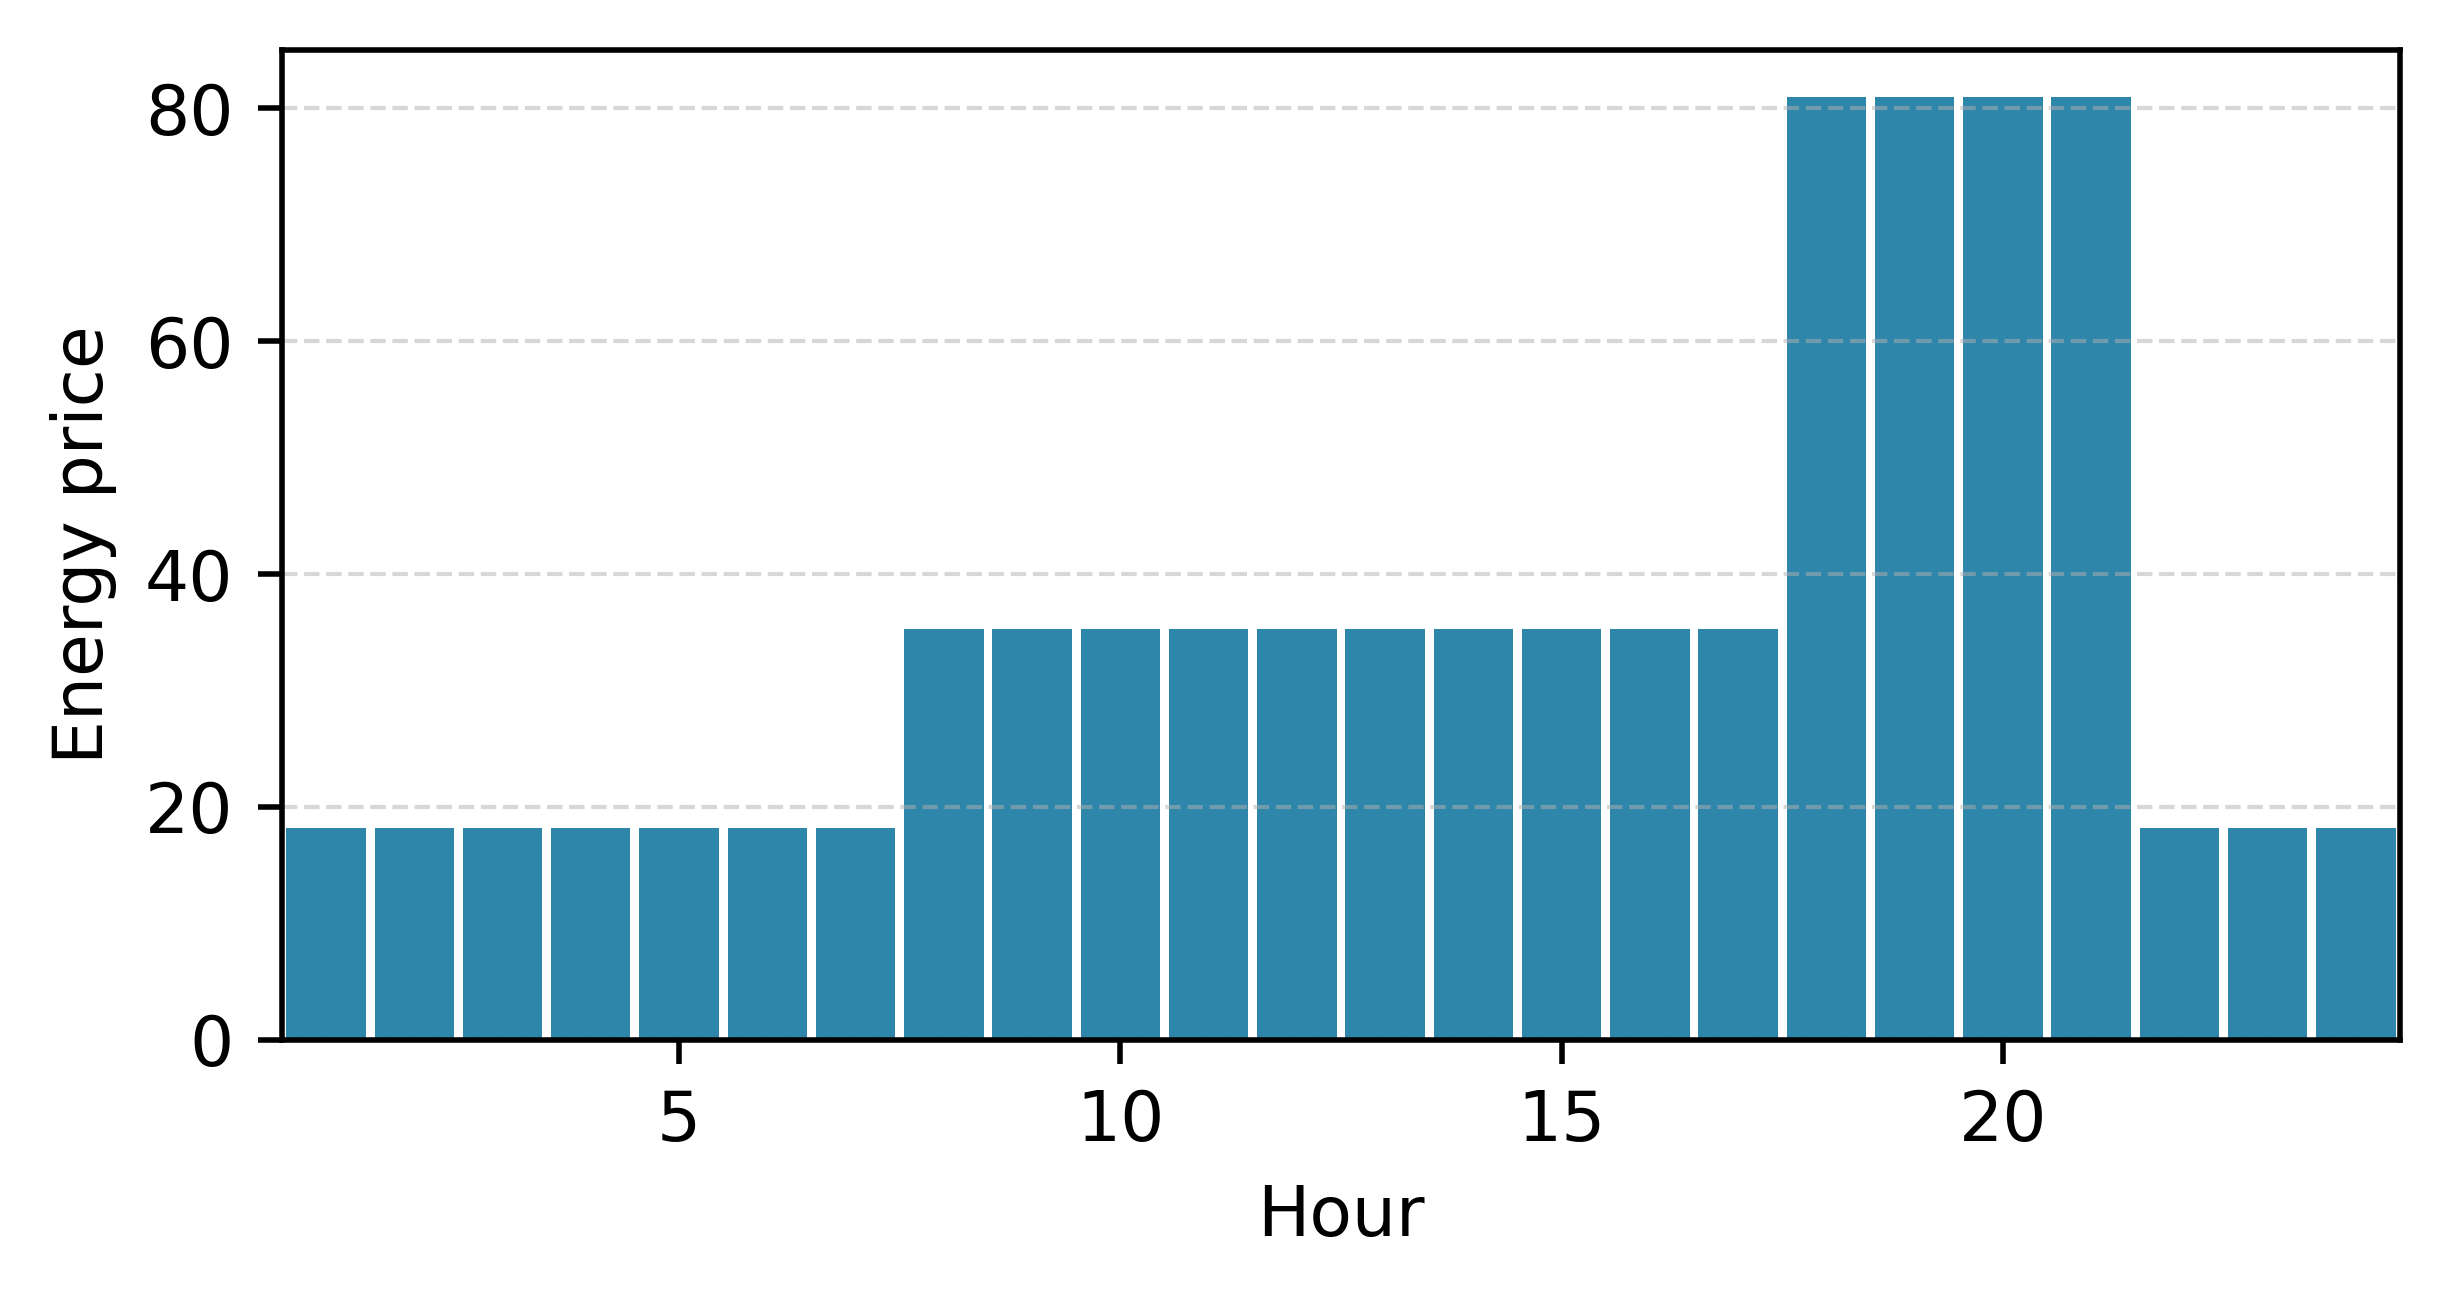
\includegraphics[width=0.9\columnwidth]{figures/Figure_4_anytown_energy_cost.png}
	\caption{Hourly energy price pattern used for pump operating cost calculations in the AnyTown Modified network.}
	\label{fig:anytown_energy_cost}
\end{figure}

\subsection{Parameter Tuning}

We tuned solver hyperparameters with Optuna \cite{Akiba2019} by sweeping the number of MPI processes ($N_{\text{procs}}$), decomposition level ($L$), and synchronization interval ($S$, the number of simulation steps between global bound exchanges) on a 16-hour instance ($NA_{\max}=2$). The best configuration was $N_{\text{procs}}=128$, $L=8$, and $S=32768$ simulation steps, and we use it for all subsequent experiments.

\subsection{Ablation Study}

We evaluated each algorithmic component by selectively disabling features on a reduced instance ($T=24$ hours, $NA_{\max}=1$) using 128 MPI processes. Table~\ref{tab:ablation} summarizes the results.

\begin{table}[htbp]
	\centering
	\caption{Ablation study results ($T=24$, $NA_{\max}=1$, $N_{\text{procs}}=128$). Slowdown shows how much slower each configuration runs compared to ``All Features'' (higher = slower).}
	\label{tab:ablation}
	\small
	\begin{tabular}{@{}lrrr@{}}
		\hline
		Configuration   & Time (s) & Slowdown     & Cost (\$) \\
		\hline
		All Features    & 5.47     & 1.0$\times$  & 3567.99   \\
		No Snapshots    & 55.47    & 10.1$\times$ & 3567.99   \\
		No Cost Pruning & 31.86    & 5.8$\times$  & 3567.99   \\
		No Pump Sorting & 3.11     & 0.6$\times$  & 3582.98   \\
		No Task Shuffle & 16.95    & 3.1$\times$  & 3567.99   \\
		\hline
	\end{tabular}
\end{table}

The snapshot mechanism is the largest contributor in our ablation, delivering a 10.1$\times$ speedup by eliminating redundant hydraulic computations during backtracking. Cost-based pruning contributes a 5.8$\times$ improvement by cutting sub-optimal branches early. Task shuffling provides a 3.1$\times$ speedup by improving load balance across processes.

Notably, disabling pump sorting yields the \emph{fastest} runtime (3.11s) because strict pruning quickly eliminates branches violating actuation constraints. This reverts to the sequential exhaustion strategy of Costa et al. However, this configuration fails to find the true optimum (\$3582.98 vs \$3567.99). LUS finds better solutions by dynamically reordering pump selection based on remaining actuation budgets, which explores regions of the search space that sequential exhaustion prunes prematurely. By preserving flexibility across all pumps, LUS maintains access to combinations that may yield lower costs later in the horizon, albeit at the expense of exploring more branches.

\subsection{Parallel Scalability}

\begin{table}[H]
	\centering
	\caption{Parallel scaling metrics ($T=24$, $NA_{\max}=1$).}
	\label{tab:scalability}
	\small
	\begin{tabular}{@{}rrrr@{}}
		\hline
		$N_{\text{procs}}$ & Time (s) & Speedup & Eff.\ (\%) \\
		\hline
		1                  & 85.08    & 1.00    & 100.0      \\
		2                  & 46.13    & 1.84    & 92.2       \\
		4                  & 23.19    & 3.67    & 91.7       \\
		8                  & 12.35    & 6.89    & 86.1       \\
		16                 & 7.47     & 11.39   & 71.2       \\
		32                 & 4.26     & 20.00   & 62.5       \\
		64                 & 3.18     & 26.76   & 41.8       \\
		128                & 3.59     & 23.69   & 18.5       \\
		\hline
	\end{tabular}
\end{table}

\begin{figure}[htbp]
	\centering
	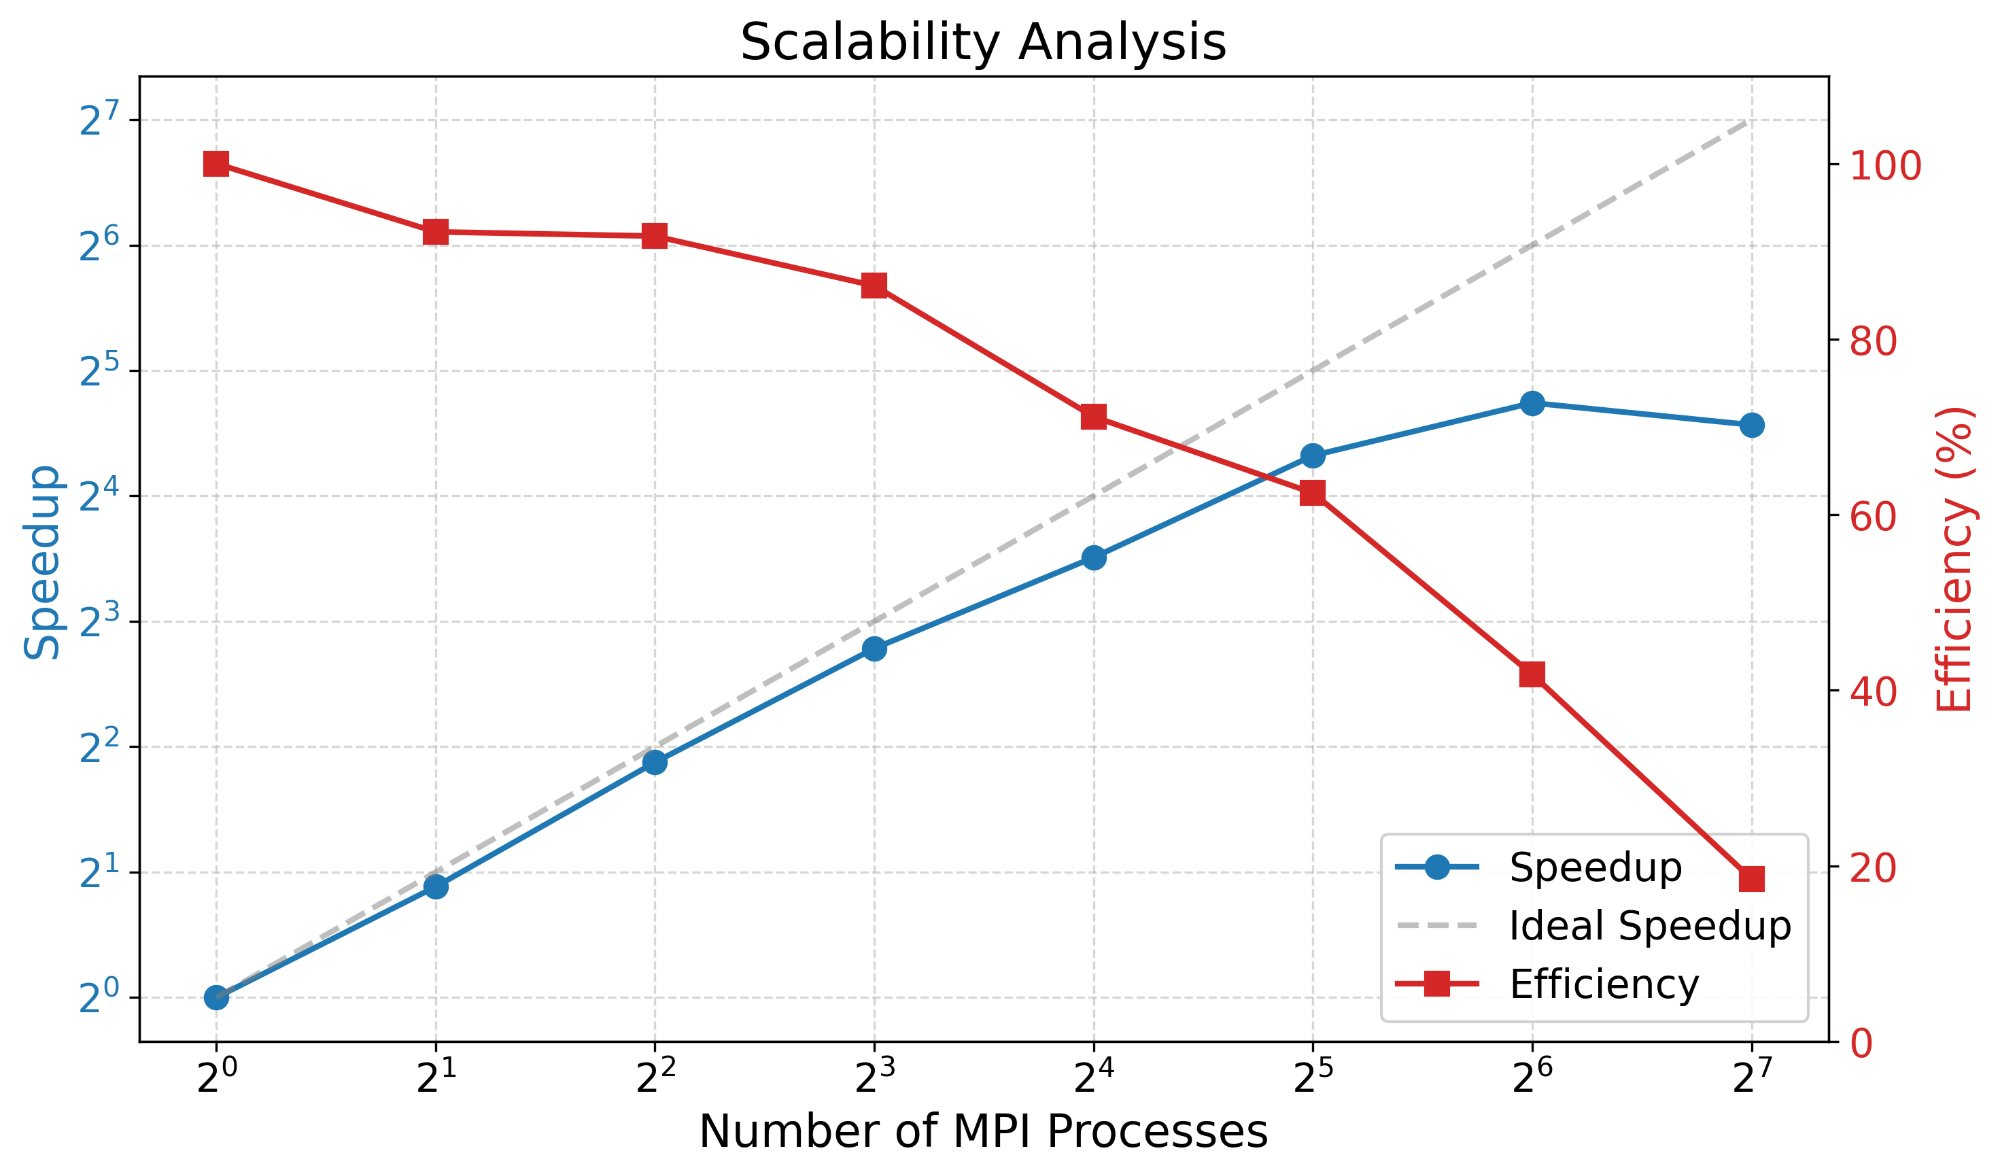
\includegraphics[width=0.9\columnwidth]{figures/Figure_5_scalability.png}
	\caption{Parallel scalability on AnyTown Modified ($T=24$, $NA_{\max}=1$).}
	\label{fig:scalability}
\end{figure}

Figure~\ref{fig:scalability} and Table~\ref{tab:scalability} present scaling results for a 24-hour instance ($NA_{\max}=1$), varying MPI processes from 1 to 128. The solver achieves 26.76$\times$ speedup with 64 processes, reducing wall-clock time from 85.08s (sequential) to 3.18s. Near-linear scaling is observed up to 8 processes (86.1\% efficiency), after which efficiency drops due to load imbalance inherent to B\&B tree pruning. The load imbalance factor, defined as $(t_{\max} - t_{\text{avg}})/t_{\text{avg}}$, grows from 8.3\% at 4 processes to 102.6\% at 64 processes. At 128 processes, performance decreases by 13\% (wall time 3.59s vs 3.18s at 64 processes) due to severe load imbalance (165.2\%), where coordination overhead exceeds the benefit of additional parallelism for this problem size. Despite this, we retain $N_{\text{procs}}=128$ for subsequent experiments because larger problem instances ($NA_{\max}=2, 3$) exhibit substantially better load balance (see Table~\ref{tab:results_24h}), where the additional processes provide meaningful speedup.

\subsection{24-Hour Optimization}

We solved the complete 24-hour problem under varying actuation constraints with $N_{\text{procs}}=128$ ($L=8$, $S=32768$). Table~\ref{tab:results_24h} presents the results, and Figure~\ref{fig:tank_levels} shows the corresponding tank level and nodal pressure trajectories over the 24-hour horizon. The figure displays tank water levels (top panel) for tanks 65, 165, and 265 with operational bounds $L_{\min}=66.53$~m and $L_{\max}=71.53$~m, and nodal pressures (bottom panel) at representative nodes 55, 90, and 170 with their respective minimum thresholds (42, 51, and 30~m). Shaded regions indicate infeasible operating ranges.

\begin{figure}[htbp]
	\centering
	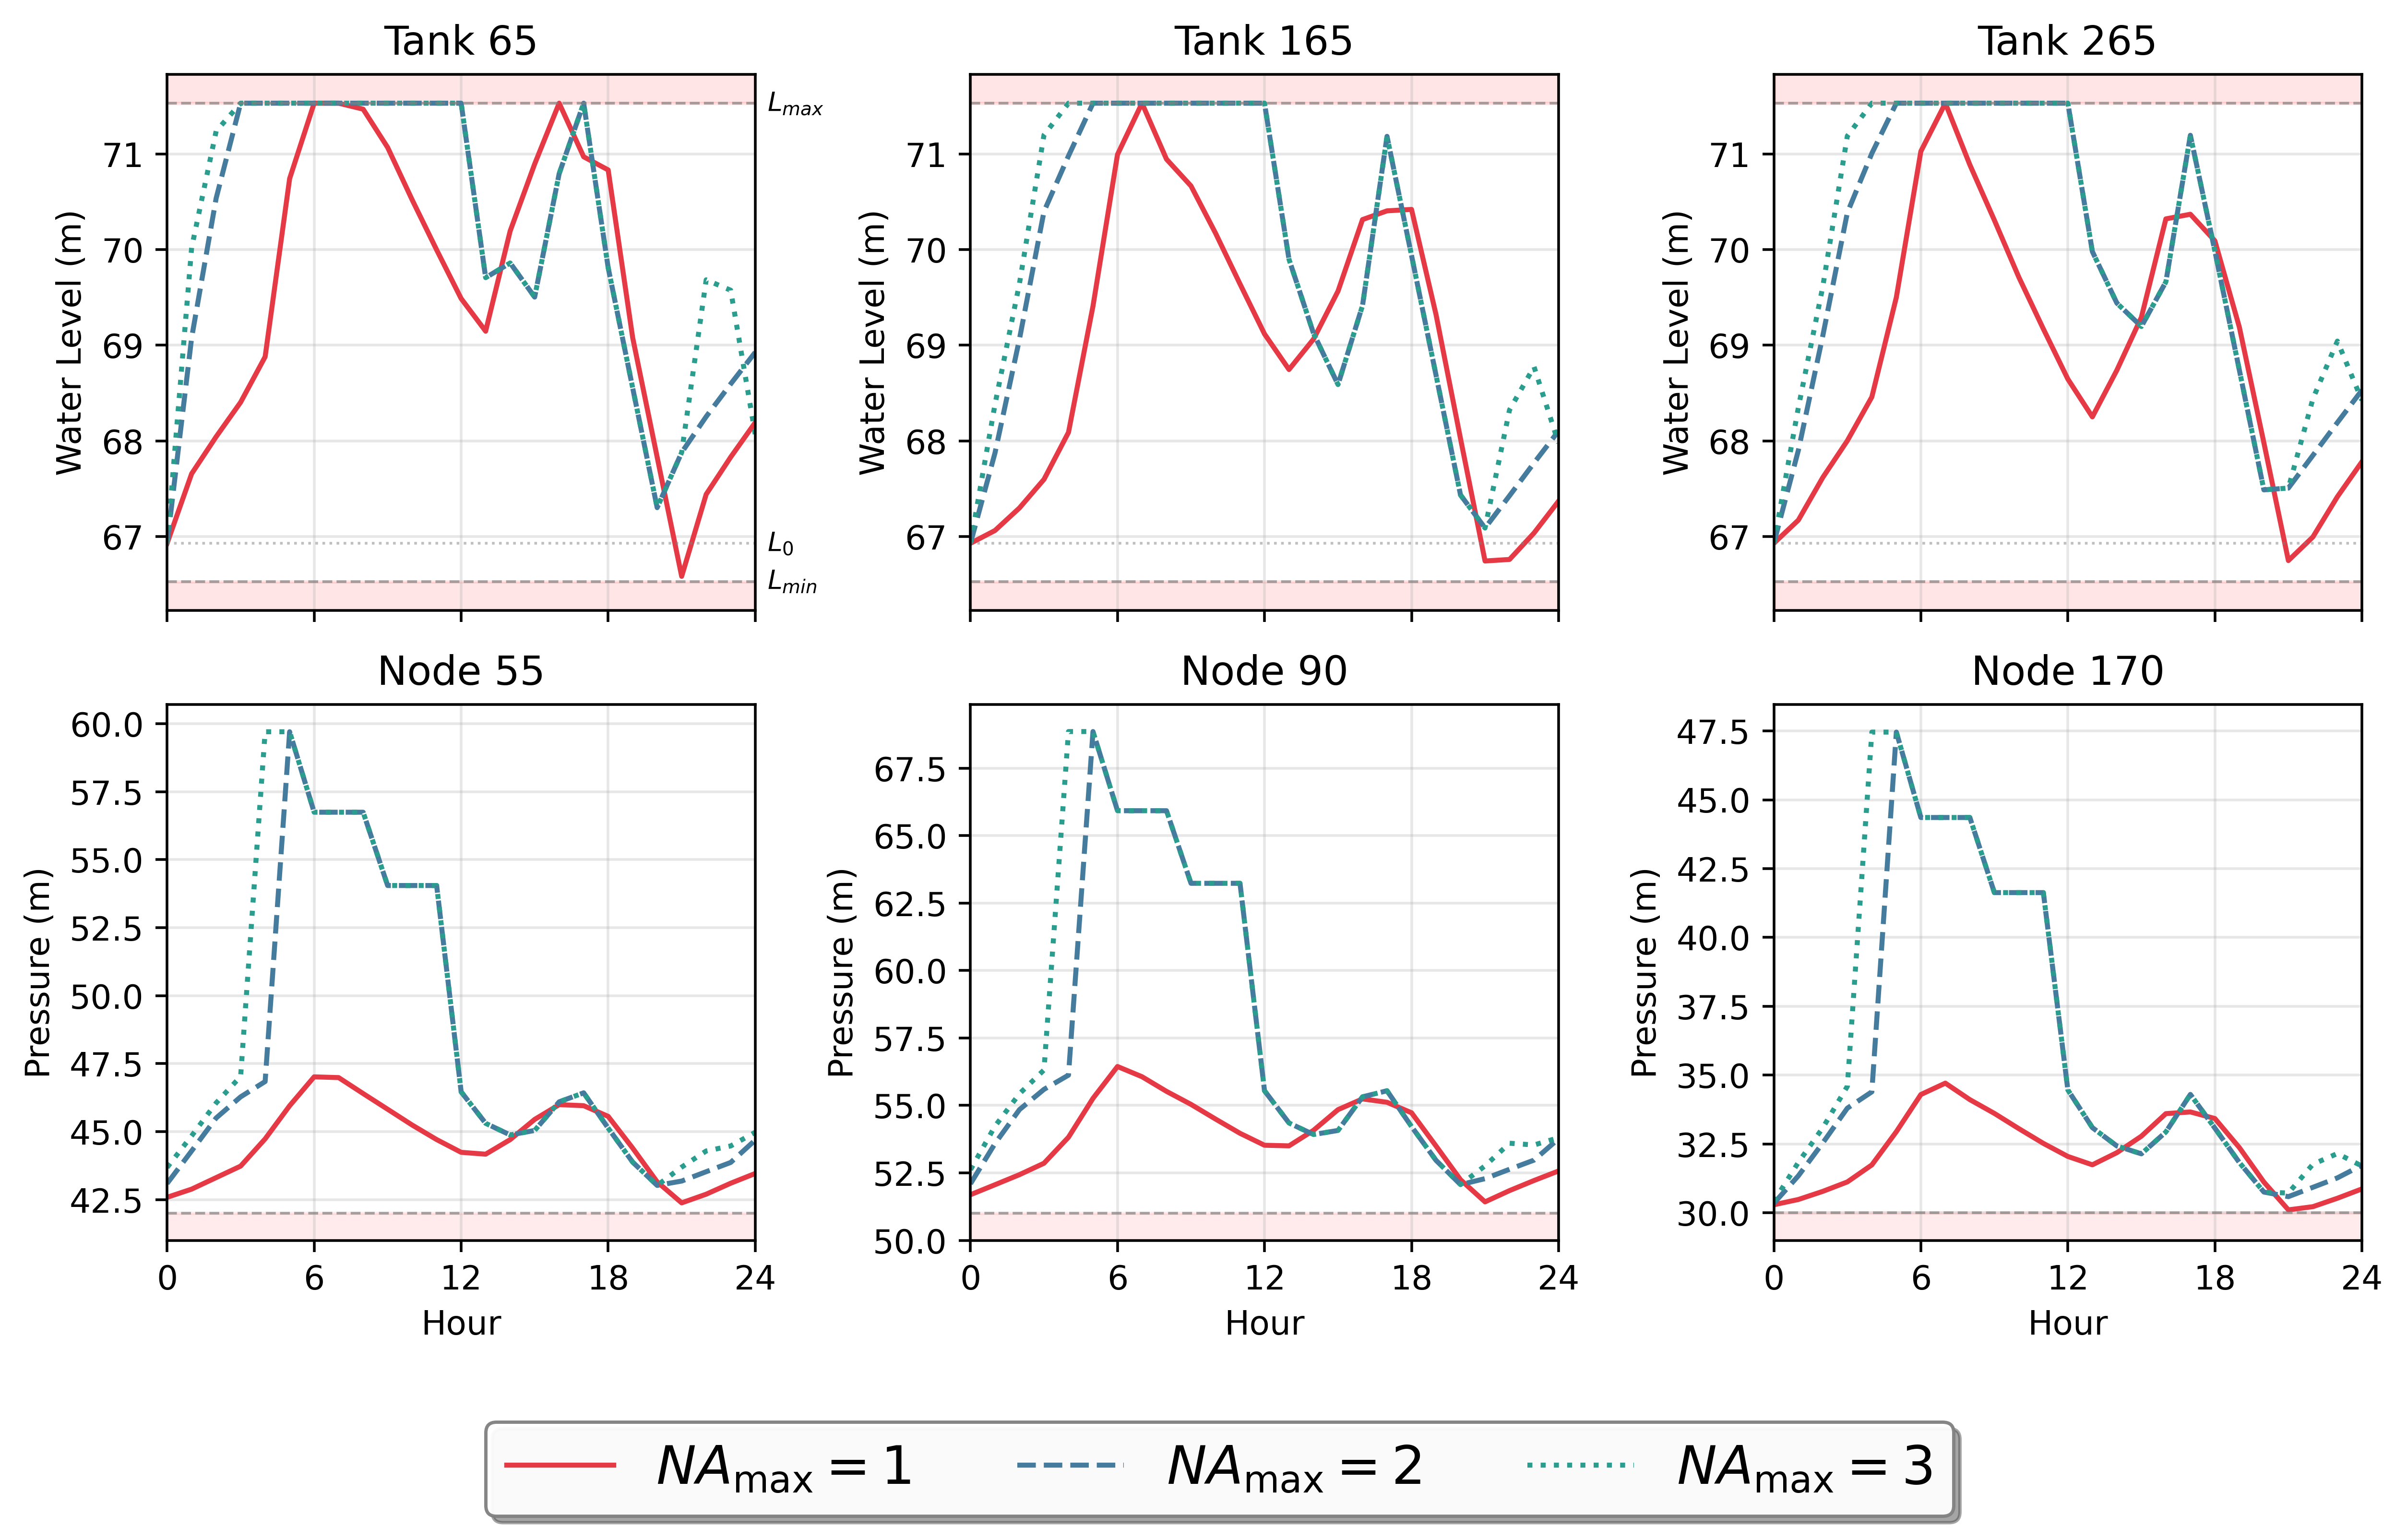
\includegraphics[width=\linewidth]{figures/Figure_6_tank_levels_24h.png}
	\caption{Hydraulic trajectories for optimal schedules under different actuation limits ($NA_{\max}=1,2,3$). Top: tank water levels; dashed lines show bounds, dotted line shows initial level. Bottom: nodal pressures; dashed lines show minimum thresholds.}
	\label{fig:tank_levels}
\end{figure}

\begin{table}[htbp]
	\centering
	\caption{Results for 24-hour optimization ($T=24$) on AnyTown Modified. Load imbalance is defined as $(t_{\max} - t_{\text{avg}})/t_{\text{avg}}$ across MPI ranks.}
	\label{tab:results_24h}
	\begin{tabular}{cccc}
		\hline
		$NA_{\max}$ & Cost (\$) & Time (s) & Load Imb.\ (\%) \\
		\hline
		1           & 3,567.99  & 3.69     & 172.0           \\
		2           & 3,472.89  & 493.11   & 23.6            \\
		3           & 3,443.46  & 10011.23 & 12.9            \\
		\hline
	\end{tabular}
\end{table}

The results reveal a clear trade-off between operational flexibility and computational cost. Restricting actuations to $NA_{\max}=1$ reduces the search space substantially, enabling solution in under 4 seconds, but at a 3.6\% higher cost (\$3,567.99) relative to the 3-actuation case. However, this configuration exhibits severe load imbalance (172.0\%), indicating that most of the search space is pruned early by actuation constraints, leaving few tasks with deep exploration. Allowing $NA_{\max}=3$ yields the lowest cost of \$3,443.46, but requires 10,011s ($\approx$2.8h). Interestingly, this configuration achieves the best load balance (12.9\% imbalance) because the larger search space distributes work more evenly across processes. The $NA_{\max}=2$ case achieves 99.1\% of the optimal cost in 4.9\% of the time required for $NA_{\max}=3$, reaching \$3,472.89 in 493s ($\approx$8.2min) with moderate imbalance (23.6\%).

\subsection{Pruning Effectiveness}

Table~\ref{tab:pruning} details the contribution of each pruning criterion to the search space reduction. The multi-criteria pruning strategy proves highly effective, eliminating 60--72\% of explored nodes before reaching terminal states.

\begin{table}[htbp]
	\centering
	\caption{Pruning statistics (\% of nodes) by constraint.}
	\label{tab:pruning}
	\footnotesize
	\begin{tabular}{@{}l*{3}{>{\centering\arraybackslash}p{1.2cm}}@{}}
		\hline
		                        & \multicolumn{3}{c}{$NA_{\max}$}  \\
		Criterion               & 1      & 2      & 3              \\
		\hline
		Actuation               & 61.9   & 43.9   & 23.7           \\
		Cost bound              & 9.1    & 19.9   & 30.0           \\
		Tank levels$^{\dagger}$ & 0.0    & 0.0    & 0.0            \\
		Pressure                & 0.8    & 3.8    & 9.0            \\
		\hline
		Total pruned            & 71.8   & 67.6   & 62.7           \\
		Feasible                & 28.2   & 32.4   & 37.3           \\
		\hline
		Nodes (total)           & 7.9M   & 1.4B   & 22.4B          \\
		\hline
		\multicolumn{4}{@{}l@{}}{\footnotesize $^{\dagger}$EPANET enforces tank bounds via head clamping; see text.}
	\end{tabular}
\end{table}

Actuation constraints dominate pruning for $NA_{\max}=1$ and $NA_{\max}=2$, accounting for up to 62\% of all explored nodes. This validates Costa et al.'s insight that tighter operational constraints improve solver performance. As actuation limits relax ($NA_{\max}=3$), cost-based pruning becomes increasingly important (30.0\%), reflecting more opportunities for the global bound to eliminate sub-optimal branches. Pressure violations also become more prominent as the search depth increases, reaching 9.0\% for $NA_{\max}=3$.

The lack of ``tank levels'' pruning is expected for this case study. In EPANET, tank levels are enforced as hydraulic boundary conditions: when a tank reaches its maximum level, its head is clamped at $L_k^{\max}$ and any additional net inflow is blocked by temporarily closing incident links, so the simulated level remains exactly at the limit rather than exceeding it. As a result, schedules that ``appear'' to keep tanks full while pumps operate do not violate the bound; the hydraulic solution simply redistributes flow and/or reduces pump flow under the higher head. Because this behavior is intrinsically handled by the simulator, an explicit pre-simulation pruning rule based on anticipated tank overfill would be both unreliable (risking false pruning) and redundant (the constraint cannot be violated in the hydraulic state). Consequently, pruning is driven primarily by actuation feasibility, cost bounds, and pressure violations.

\subsection{Comparative Analysis}

We compare our framework with the sequential B\&B of Costa et al. \cite{Costa2016}, the Genetic Algorithm of Cimorelli et al. \cite{Cimorelli2020}, and the Digital Harmony Search (DHS) of De Paola et al. \cite{Paola2024} on AnyTown Modified. All reference solutions were re-evaluated using EPANET~3.0 to ensure consistency; each remained hydraulically feasible with costs matching original reports within 0.1\% (differences attributable to minor variations between EPANET~2 and EPANET~3 hydraulic engines).

Figures~\ref{fig:comparison_a1}--\ref{fig:comparison_a3} present detailed pump schedules for all methods at each actuation limit. These visualizations show that our schedules differ from prior approaches in pump timing and activation sequences while achieving superior cost performance.

Our EPANET-BB framework achieves the lowest cost across all actuation limits tested, improving upon both exact and meta-heuristic methods. For $NA_{\max}=1$, EPANET-BB finds \$3,567.99, reducing costs by 1.8\% compared to Cimorelli et al.'s GA (\$3,634.67). For $NA_{\max}=2$, our solution (\$3,472.89) improves by 3.0\% over Cimorelli et al. (\$3,580.11). For $NA_{\max}=3$, EPANET-BB achieves \$3,443.46, a 3.7\% improvement over Cimorelli et al.'s best-reported result (\$3,575.54). These improvements demonstrate the value of exhaustive search with effective pruning.

Computational performance shows substantial improvement over sequential B\&B: speedups of 29$\times$ to 115$\times$ were observed compared to Costa et al.'s implementation. The most constrained case ($NA_{\max}=1$) reduced computation time from 425 seconds to 3.69 seconds (115$\times$ speedup). The moderately constrained case ($NA_{\max}=2$) decreased from 10.3 hours to 8.2 minutes (75$\times$ speedup). The least constrained case ($NA_{\max}=3$) reduced computation from 81 hours to 2.8 hours (29$\times$ speedup). These performance enhancements demonstrate that exact optimization can be applied within sub-hour to few-hour timeframes suitable for day-ahead operational planning, offering theoretical guarantees that are not inherent to meta-heuristic approaches.


\begin{figure*}[htbp]
	\centering
	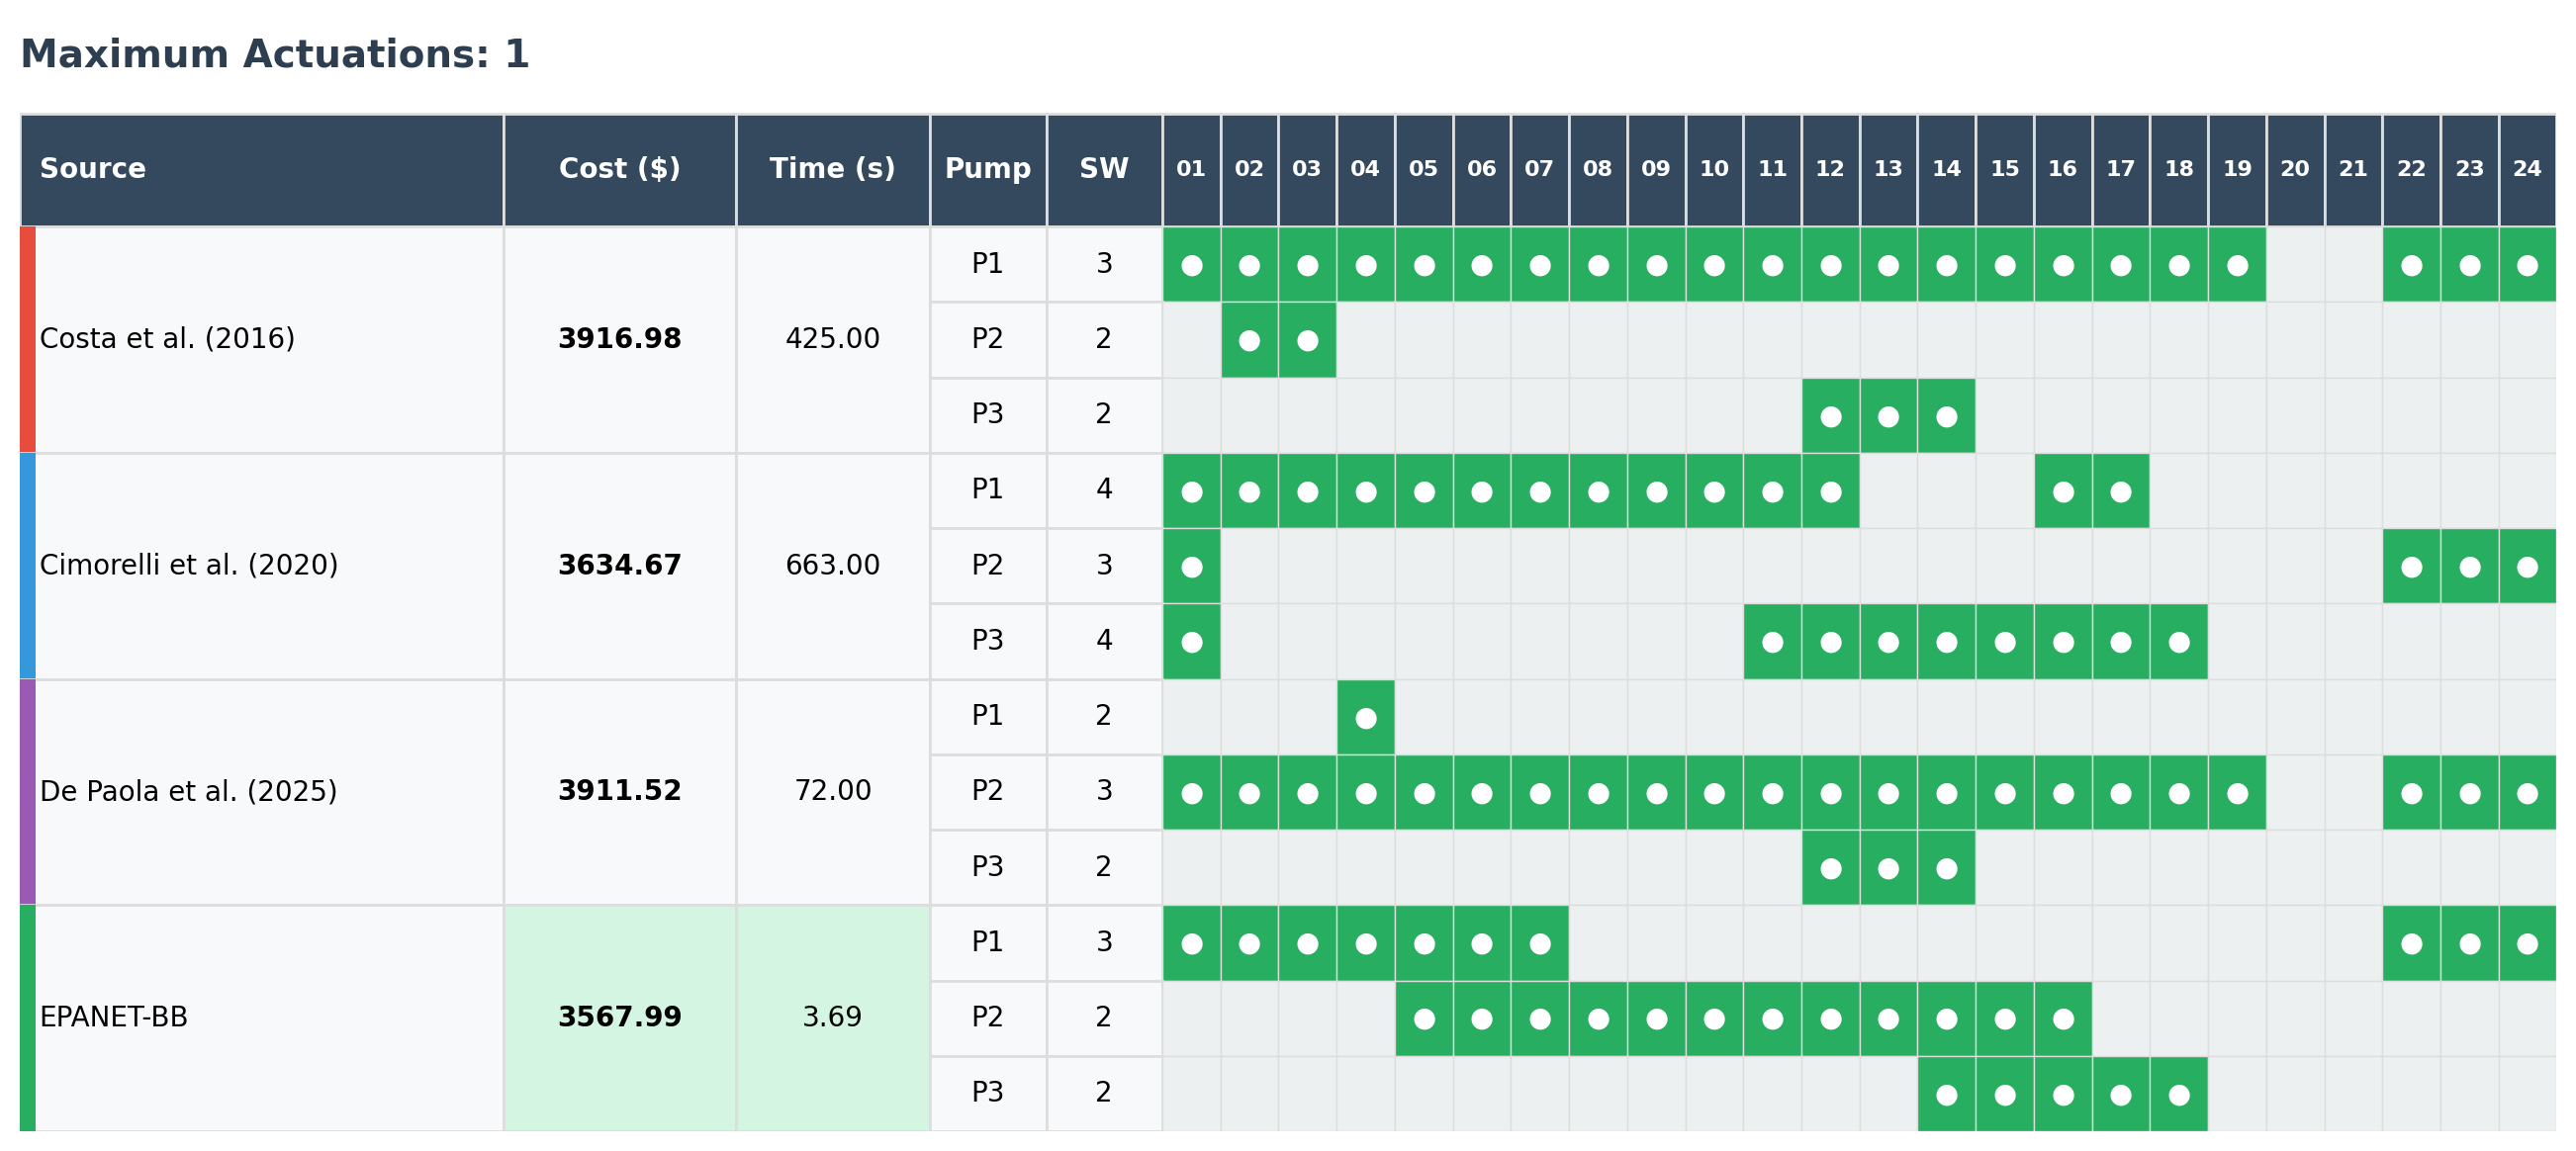
\includegraphics[width=\textwidth]{figures/Figure_7_comparison_table_a1.png}
	\caption{Pump schedule comparison for $NA_{\max}=1$. EPANET-BB achieves the lowest cost (\$3,567.99), improving upon Cimorelli et al.'s GA (\$3,634.67) by 1.8\%.}
	\label{fig:comparison_a1}
\end{figure*}

\begin{figure*}[htbp]
	\centering
	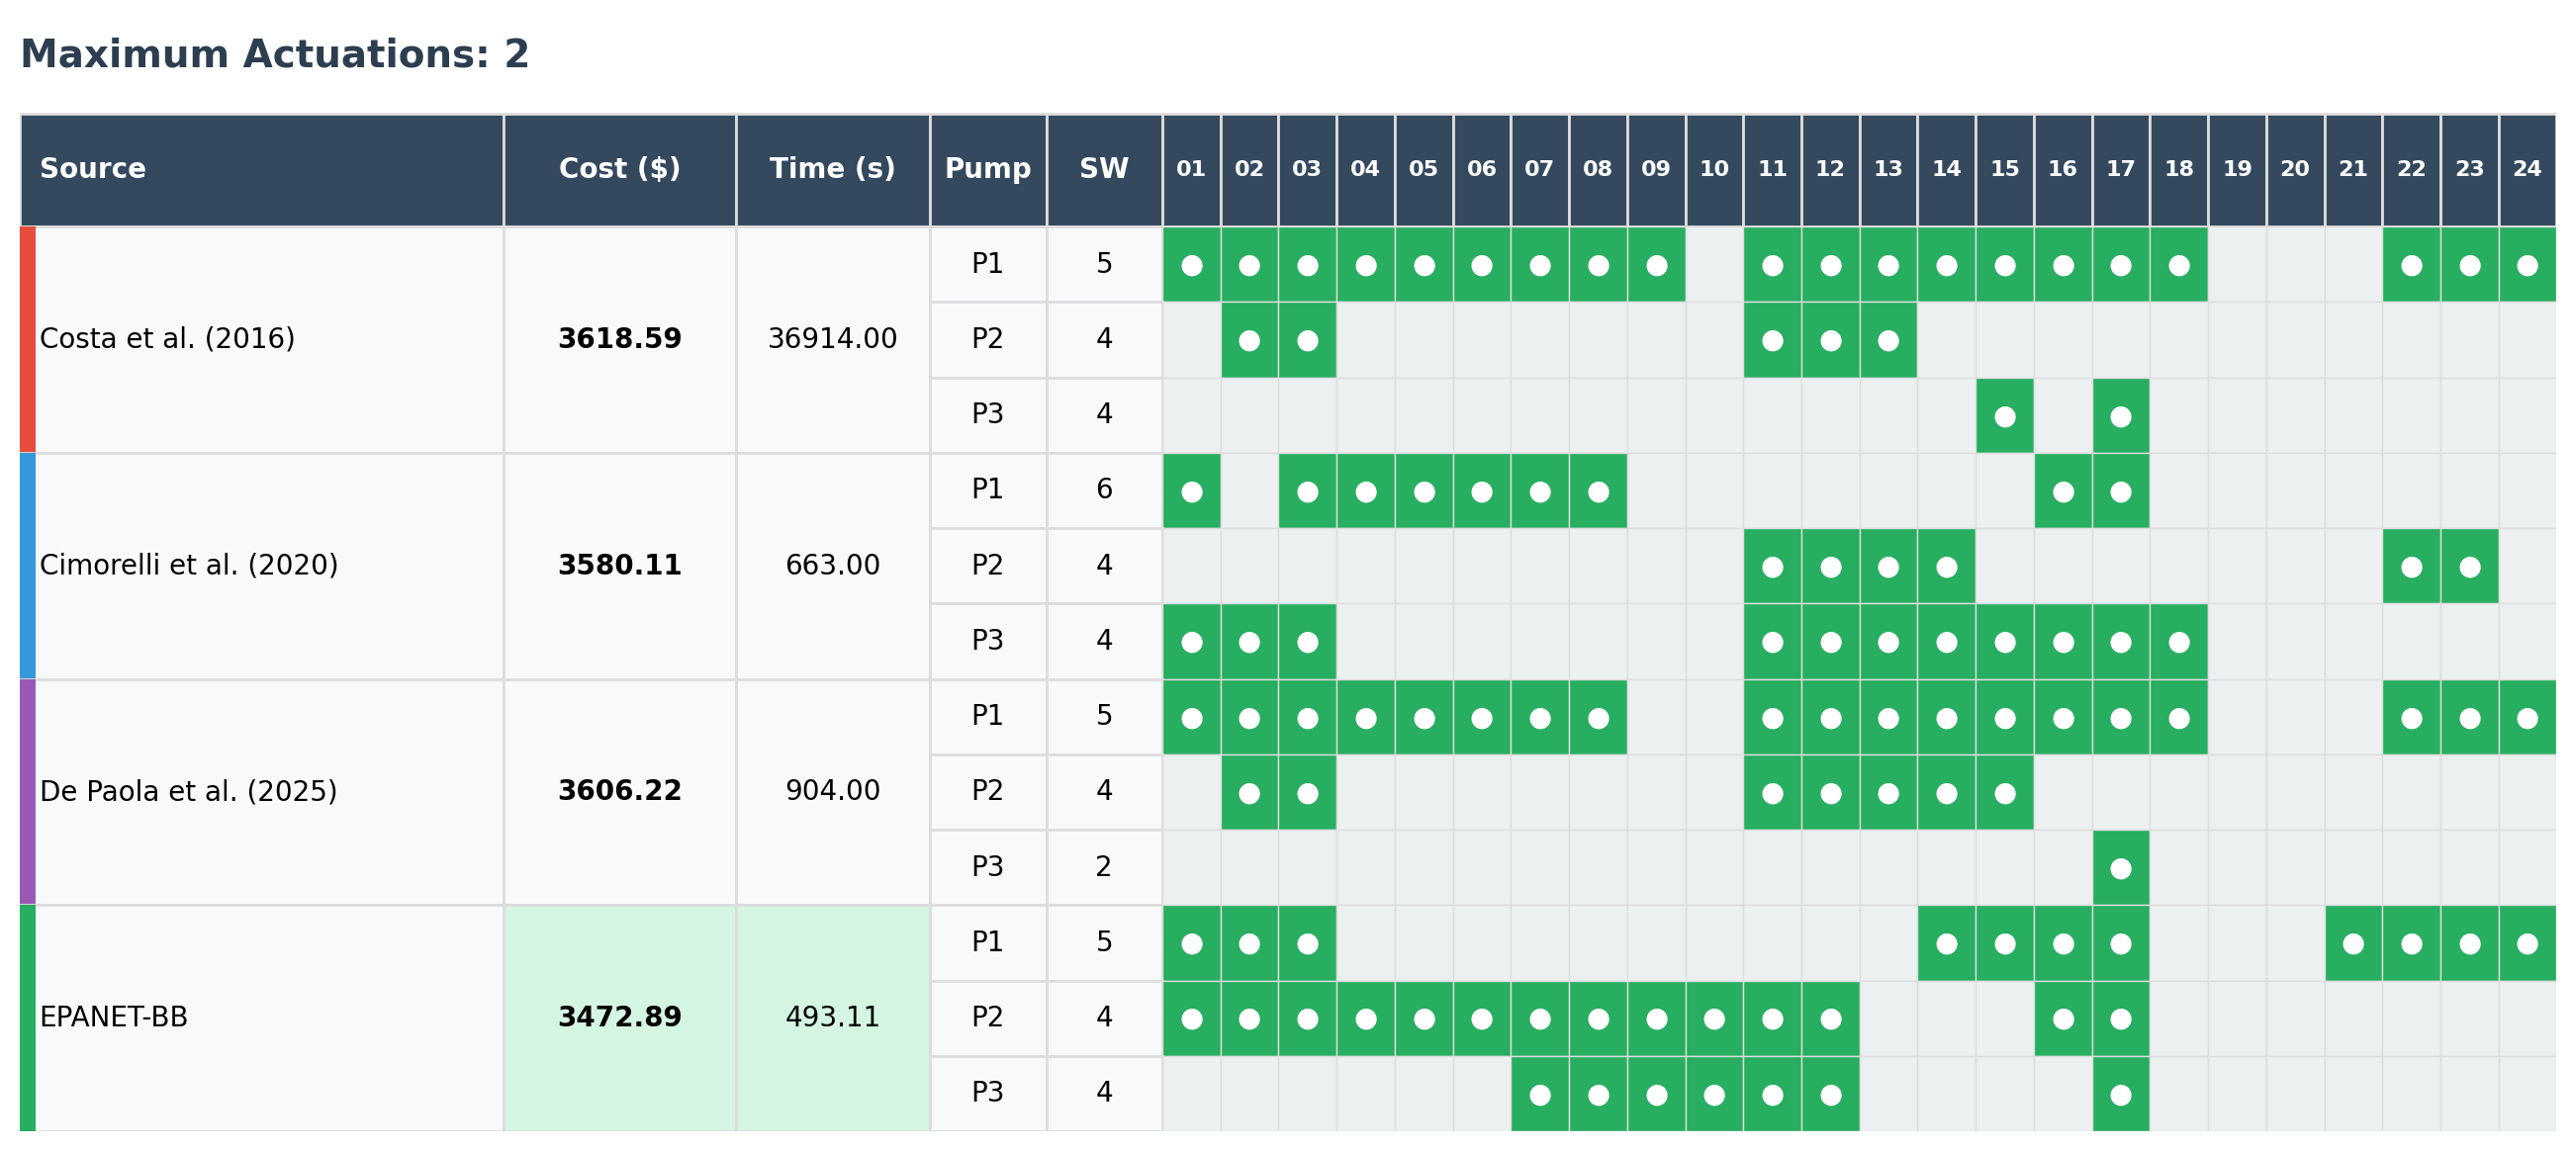
\includegraphics[width=\textwidth]{figures/Figure_8_comparison_table_a2.png}
	\caption{Pump schedule comparison for $NA_{\max}=2$. EPANET-BB achieves the lowest cost (\$3,472.89), improving upon Cimorelli et al.'s GA (\$3,580.11) by 3.0\%.}
	\label{fig:comparison_a2}
\end{figure*}

\begin{figure*}[htbp]
	\centering
	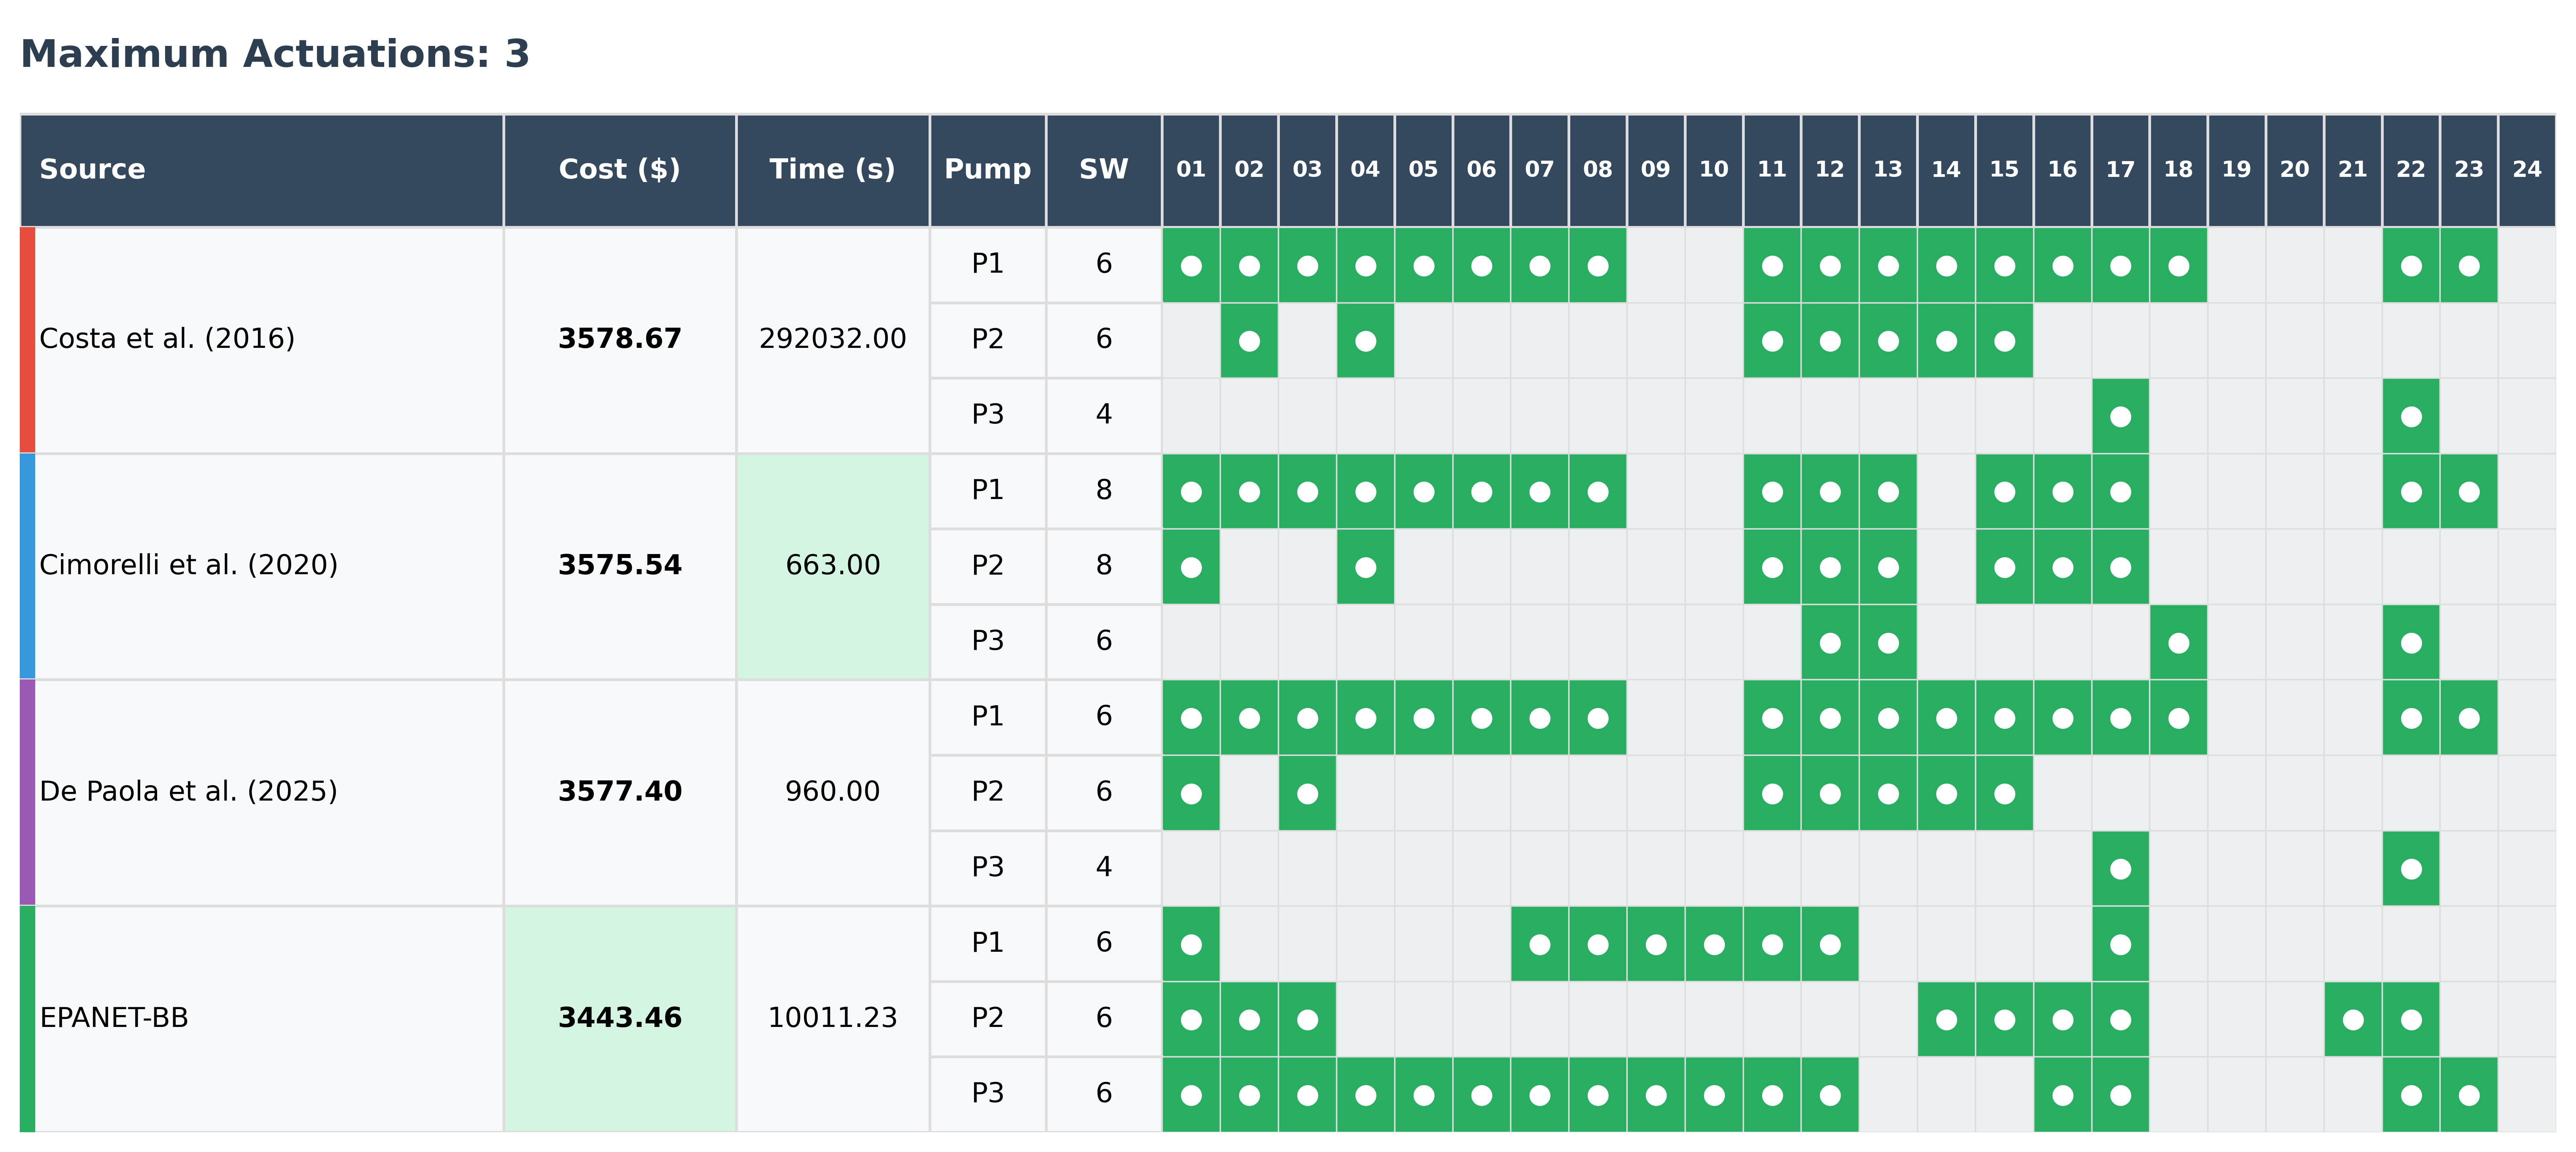
\includegraphics[width=\textwidth]{figures/Figure_9_comparison_table_a3.png}
	\caption{Pump schedule comparison for $NA_{\max}=3$. EPANET-BB achieves the lowest cost (\$3,443.46), improving upon Cimorelli et al.'s GA (\$3,575.54) by 3.7\%.}
	\label{fig:comparison_a3}
\end{figure*}

\subsection{Discussion}

Our results reveal several noteworthy findings and limitations that merit discussion.

\textbf{LUS Trade-off.} The ablation study uncovered an unexpected trade-off: disabling pump sorting (LUS) produces the fastest runtime but yields suboptimal solutions. This occurs because sequential exhaustion aggressively prunes the search space by depleting each pump's actuation budget before considering alternatives, which happens to align well with the pruning criteria but misses better configurations that require distributing actuations across pumps. LUS sacrifices some pruning efficiency to maintain flexibility, ultimately finding the global optimum at modest computational cost.

\textbf{Scalability Considerations.} The AnyTown Modified network has three pumps, yielding a search space of $4^{24} \approx 2.8 \times 10^{14}$ high-level configurations for the full 24-hour problem. Networks with more pumps will face exponentially larger search spaces. Our framework's effectiveness depends critically on the actuation constraint $NA_{\max}$, which provides the dominant pruning mechanism. For networks where operational constraints are looser, additional strategies such as bound tightening, symmetry breaking, or hierarchical decomposition may be necessary.

\textbf{Parallel Efficiency.} Load imbalance remains the primary barrier to parallel efficiency, degrading from 86\% at 8 processes to 42\% at 64 processes for the $NA_{\max}=1$ case. Interestingly, larger problem instances ($NA_{\max}=3$) achieve better load balance (12.9\% imbalance) because the search space is more uniformly distributed. Dynamic work stealing could improve efficiency for highly constrained instances where static decomposition produces uneven subtrees.

\textbf{Generalizability.} While our experiments focus on a single benchmark network, the algorithmic innovations---snapshot persistence, LUS, and cooperative pruning---are network-agnostic and should transfer to other fixed-speed pump scheduling problems. Variable-speed pumps introduce continuous decision variables that would require different solution approaches.

\section{Conclusion}

We presented a high-performance Branch-and-Bound framework for pump scheduling in water distribution networks. Our three key innovations are MPI-based parallelism, hydraulic snapshot persistence, and balanced pump selection via LUS. These bridge the gap between theoretical optimality and practical applicability.

Our experiments demonstrate that exact optimization of 24-hour pump schedules is now feasible in operational timeframes. The solver achieves speedups of 29--115$\times$ over sequential implementations, reducing computation from hours to minutes while maintaining optimality guarantees. Notably, our results improve upon the best-known solutions from meta-heuristics, achieving \$3,443.46 for $NA_{\max}=3$---a 3.7\% improvement over Cimorelli et al.'s GA result (\$3,575.54). The ablation study confirms that snapshot persistence delivers the most significant performance gain (10.1$\times$), validating our focus on eliminating redundant hydraulic simulations.

Two directions merit further investigation. First, dynamic work stealing could improve parallel efficiency beyond the 42\% observed at 64 processes by addressing load imbalance inherent to B\&B tree exploration. Second, extending the framework to larger networks with more pumps will require additional pruning strategies or hierarchical decomposition to manage the exponential growth in search space.

\section*{Code Availability}

The source code and data required to reproduce the results presented in this work are available in the following GitHub repository: \url{https://github.com/michaelsouza/epanet-bb}.

\section*{Funding}
This research was partially funded by the Brazilian research agencies FAPESP (Grant Nos. 2013/07375-0, 2023/08706-1, and 2024/00923-6) and CNPq (Grant Nos. 305227/2022-0, 404616/2024-0, and 402609/2025-5).
Michael Ferreira de Souza, Albert Einstein Fernandes Muritiba, and Asc\^anio Dias Ara\'ujo acknowledge financial support from CAPES (Coordenação de Aperfeiçoamento de Pessoal de Nível Superior), CNPq (Conselho Nacional de Desenvolvimento Científico e Tecnológico), and FUNCAP (Fundação Cearense de Apoio ao Desenvolvimento Científico e Tecnológico).
J\'essica Gomes Melo da Rocha acknowledges a Master’s scholarship from FUNCAP.
The funding agencies had no role in the study design; data collection, analysis, or interpretation; manuscript preparation; or the decision to submit the article for publication.

\section*{Declaration of competing interests}
The authors declare that they have no known competing financial interests or
personal relationships that could have appeared to influence the work reported
in this paper.

\section*{Declaration of generative AI and AI-assisted technologies in the manuscript preparation process}
During the preparation of this work, the authors used an AI-assisted language model (Claude, Anthropic) to improve readability, clarity, and
professionalism in writing.
After using this tool/service, the authors reviewed and edited the content as
needed and take full responsibility for the content of the published article.

\printcredits

%% Loading bibliography style file
\bibliographystyle{model1-num-names}
%\bibliographystyle{cas-model2-names}

% Loading bibliography database
\bibliography{cas-refs}


%\vskip3pt

\end{document}